%% LyX 2.3.4.2 created this file.  For more info, see http://www.lyx.org/.
%% Do not edit unless you really know what you are doing.
% \documentclass[english,dvipsnames,aspectratio=169]{beamer}
\documentclass[english,dvipsnames,aspectratio=169,handout]{beamer}
\usepackage{mathptmx}
\usepackage{eulervm}
\usepackage[T1]{fontenc}
\usepackage[latin9]{inputenc}
\usepackage{babel}
\usepackage{amstext}
\usepackage{amssymb}
\usepackage{graphicx}
\usepackage{ifthen}
\usepackage{xcolor}
\usepackage{xspace}
\usepackage{tikz}
\usetikzlibrary{tikzmark}
\usetikzlibrary{calc}
\usepackage{pgfplots}
%\pgfplotsset{compat=1.17}
\usepackage{booktabs}
\usepackage{xpatch}
\usepackage{multirow}
\usepackage{colortbl}
\usepackage{pgfpages}
\usepackage{bbm}

\xpatchcmd{\itemize}
  {\def\makelabel}
  {\ifnum\@itemdepth=1\relax
     \setlength\itemsep{2ex}% separation for first level
   \else
     \ifnum\@itemdepth=2\relax
       \setlength\itemsep{1ex}% separation for second level
     \else
       \ifnum\@itemdepth=3\relax
         \setlength\itemsep{0.5ex}% separation for third level
   \fi\fi\fi\def\makelabel
  }
 {}
 {}

\ifx\hypersetup\undefined
  \AtBeginDocument{%
    \hypersetup{unicode=true,pdfusetitle,
 bookmarks=true,bookmarksnumbered=false,bookmarksopen=false,
 breaklinks=false,pdfborder={0 0 0},pdfborderstyle={},backref=false,colorlinks=true,
 allcolors=NYUPurple,urlcolor=LightPurple}
  }
\else
  \hypersetup{unicode=true,pdfusetitle,
 bookmarks=true,bookmarksnumbered=false,bookmarksopen=false,
 breaklinks=false,pdfborder={0 0 0},pdfborderstyle={},backref=false,colorlinks=true,
 allcolors=NYUPurple,urlcolor=LightPurple}
\fi

\makeatletter

%%%%%%%%%%%%%%%%%%%%%%%%%%%%%% LyX specific LaTeX commands.
%% Because html converters don't know tabularnewline
\providecommand{\tabularnewline}{\\}

%%%%%%%%%%%%%%%%%%%%%%%%%%%%%% Textclass specific LaTeX commands.
% this default might be overridden by plain title style
\newcommand\makebeamertitle{\frame{\maketitle}}%
% (ERT) argument for the TOC
\AtBeginDocument{%
  \let\origtableofcontents=\tableofcontents
  \def\tableofcontents{\@ifnextchar[{\origtableofcontents}{\gobbletableofcontents}}
  \def\gobbletableofcontents#1{\origtableofcontents}
}

%%%%%%%%%%%%%%%%%%%%%%%%%%%%%% User specified LaTeX commands.
\usetheme{CambridgeUS} 
\beamertemplatenavigationsymbolsempty


% Set Color ==============================
\definecolor{NYUPurple}{RGB}{87,6,140}
\definecolor{LightPurple}{RGB}{165,11,255}


\setbeamercolor{title}{fg=NYUPurple}
\setbeamercolor{frametitle}{fg=NYUPurple}

\setbeamercolor{background canvas}{fg=NYUPurple, bg=white}
\setbeamercolor{background}{fg=black, bg=NYUPurple}

\setbeamercolor{palette primary}{fg=black, bg=gray!30!white}
\setbeamercolor{palette secondary}{fg=black, bg=gray!20!white}
\setbeamercolor{palette tertiary}{fg=gray!20!white, bg=NYUPurple}

\setbeamertemplate{headline}{}
\setbeamerfont{itemize/enumerate body}{}
\setbeamerfont{itemize/enumerate subbody}{size=\normalsize}

\setbeamercolor{parttitle}{fg=NYUPurple}
\setbeamercolor{sectiontitle}{fg=NYUPurple}
\setbeamercolor{sectionname}{fg=NYUPurple}
\setbeamercolor{section page}{fg=NYUPurple}
%\setbeamercolor{description item}{fg=NYUPurple}
%\setbeamercolor{block title}{fg=NYUPurple}

\setbeamertemplate{blocks}[rounded][shadow=false]
\setbeamercolor{block body}{bg=normal text.bg!90!NYUPurple}
\setbeamercolor{block title}{bg=NYUPurple!30, fg=NYUPurple}



\AtBeginSection[]{
  \begin{frame}
  \vfill
  \centering
\setbeamercolor{section title}{fg=NYUPurple}
 \begin{beamercolorbox}[sep=8pt,center,shadow=true,rounded=true]{title}
    \usebeamerfont{title}\usebeamercolor[fg]{title}\insertsectionhead\par%
  \end{beamercolorbox}
  \vfill
  \end{frame}
}

\makeatother

\setlength{\parskip}{\medskipamount} 

\input ../macros

\begin{document}
\input ../rosenberg-macros

%\setbeameroption{show notes on second screen}

\title[CSCI-GA]{Neural Networks II: Deep Learning}
\author[]{Mengye Ren
\\ \quad\\
\small (Slides credit to David Rosenberg, He He, et al.)}
% \author{He He \\
% Slides based on Lecture
% \href{https://github.com/davidrosenberg/mlcourse/blob/gh-pages/Lectures/13a.k-means.pdf}{13a} from David Rosenberg's course materials (\url{https://github.com/davidrosenberg/mlcourse})
% }
\date[]{Nov 26, 2024}
\institute[]{NYU}

\makebeamertitle
\mode<article>{Just in article version}

\begin{frame}{Slides}
\begin{center}

\includegraphics[width=0.4\textwidth]{figures/qr_11.png}
\end{center}
\end{frame}

\begin{frame}{Logistics}
\begin{itemize}
    \item Homework 4 Due: Dec 3.
    \item Last lecture: Dec 10 Project presentation. 
    \item Presentation order: Your assigned Group ID.
    \item Each group has a max of 4 minutes (hard stop) + 1 min Q\&A.
\end{itemize}
\end{frame}

% \begin{frame}{Fully connected vs. locally connected}
% \begin{itemize}
%     \item So far we apply a layer where all output neurons are connected to all input neurons.
%     \item In matrix form, $\mathbf{z} = W \mathbf{x}$.
%     \item This is also called a fully connected layer or a dense layer or a linear layer.
%     \pause
%     \item For $200 \times 200$ image and 1000 hidden units, the matrix of a single layer will have 40M parameters!
% \end{itemize}
% \begin{center}
% 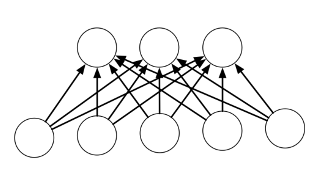
\includegraphics[width=0.34\textwidth]{figures/fully_connected.png}
% 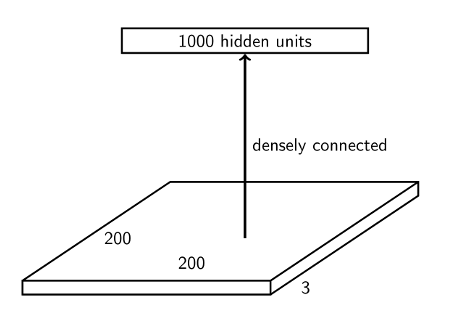
\includegraphics[width=0.34\textwidth]{figures/nn_1000_hidden.png}
% \end{center}
% \end{frame}
% \begin{frame}{Fully connected vs. locally connected}
% \begin{itemize}
%     \item An alternative strategy is to use local connection.
%     \item For neuron i, only connects to its neighborhood (e.g. [i+k, i-k])
%     \item For images, we index neurons with three dimensions i, j, and c.
%     \item i = vertical index, j = horizontal index, c = channel index.
% \end{itemize}
% \begin{center}
% 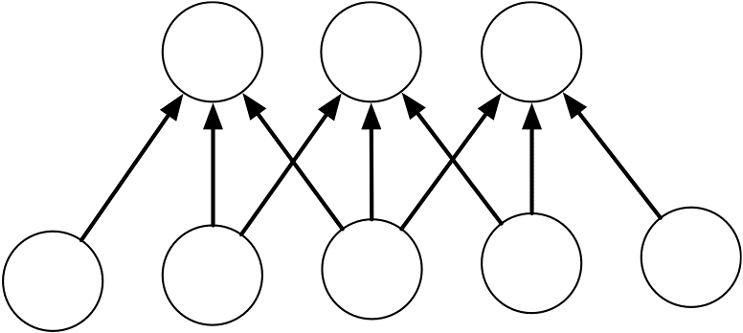
\includegraphics[width=0.3\textwidth]{figures/locally_connected.png}
% 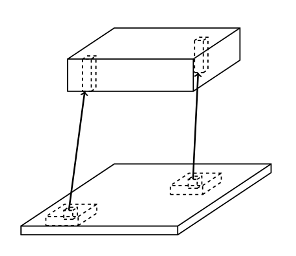
\includegraphics[width=0.3\textwidth]{figures/locally_connected_3d.png}
% \end{center}
% \end{frame}

\begin{frame}{Local connection patterns}
\begin{columns}
\begin{column}{0.65\textwidth}
\begin{itemize}
    \onslide<1->{\item The typical image input layer has 3 channels R G B for color or 1 channel for grayscale.
    \item The hidden layers may have $C$ channels, at each spatial location $(i, j)$.
    }
    \onslide<2->{
    \item Now each hidden neuron $z_{i,j,c}$ receives inputs from $x_{i \pm k, j \pm k, \cdot}$ 
    % - taking all the channels at neighboring spatial locations.
    \item $k$ is the ``kernel'' size - do not confuse with the other kernel we learned.
    \item $z_{i,j,c} = \sum_{i'\in[i\pm k], j' \in [j \pm k], c'} x_{i'j'c'} \textcolor{red}{w_{i, j, i'-i, j'-j, c',c}}$
    }
    \onslide<3->{
    \item The spatial awareness (receptive field) of the neighborhood grows bigger as we go deeper.
    }
\end{itemize}
\end{column}
\begin{column}{0.34\textwidth}
\begin{center}
\onslide<1->{
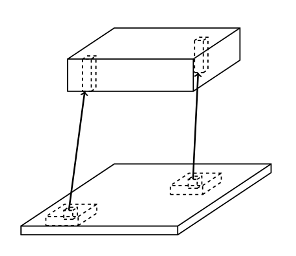
\includegraphics[width=0.8\textwidth]{figures/locally_connected_3d.png}
}
\end{center}
\end{column}
\end{columns}
\end{frame}

\begin{frame}{Weight sharing}
\begin{itemize}
\item Still a lot of weights: If we have 100 channels in the second layer, then $200 \times 200 \times 3 \times 100 = 12M$
\pause
\item Local information is the same regardless of the position of an element.
% \item E.g. A dog is a dog anywhere in an image.
\pause
\item Solution: We can tie the weights at different locations.
\end{itemize}
\begin{center}
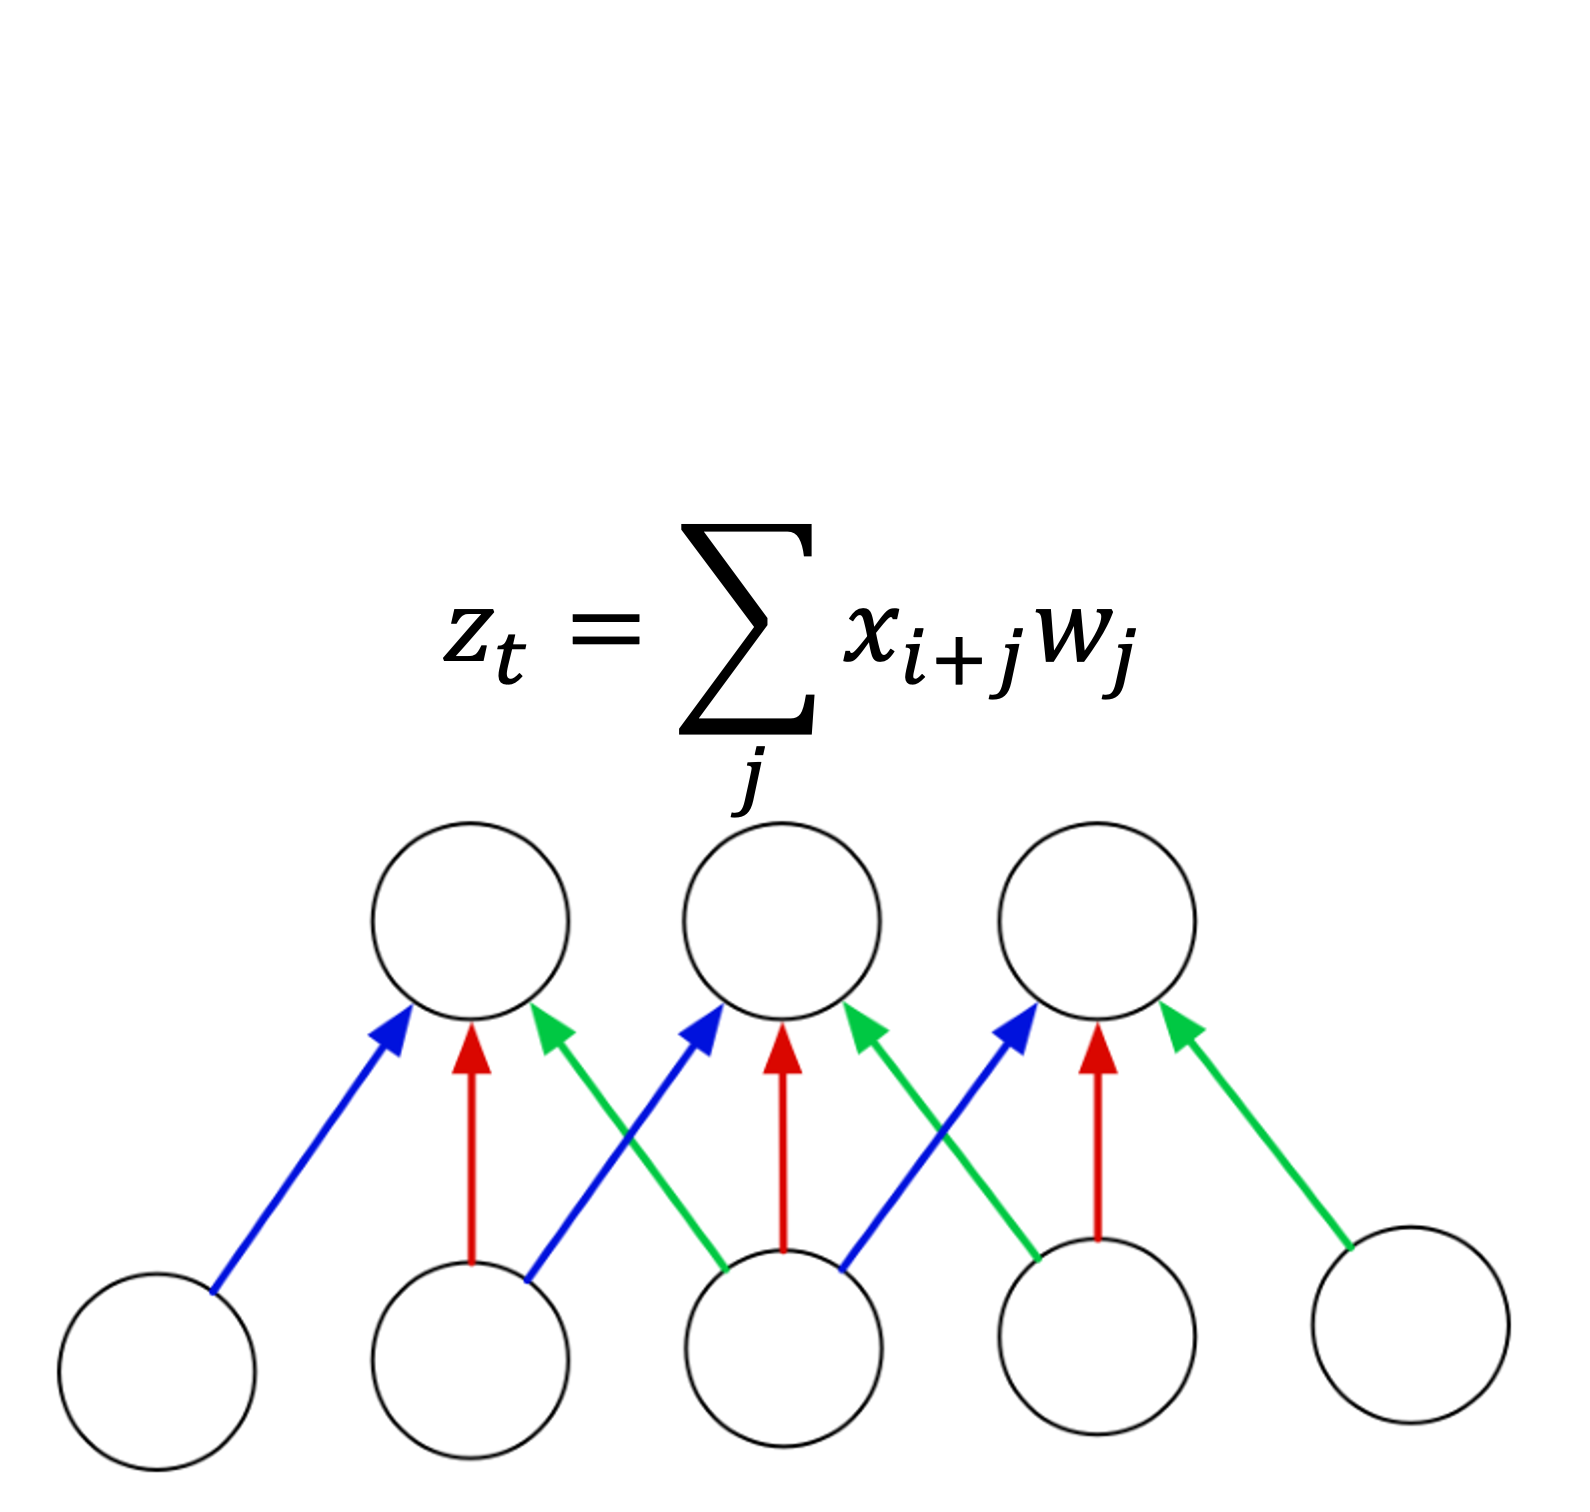
\includegraphics[width=0.3\textwidth,trim={0 0 0 6.2cm},clip]{figures/weight_share_2d.png}
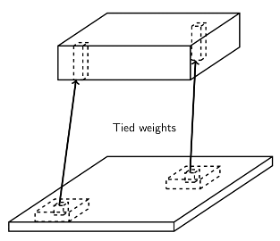
\includegraphics[width=0.3\textwidth]{figures/weight_share_3d.png}
\end{center}
\end{frame}

\begin{frame}{2D convolution}

\begin{columns}
\begin{column}{0.5\textwidth}
\begin{itemize}
    \item Using the same weight connections for each activation spatial location works like the ``filtering operation'' or ``convolution''
    \item The neighborhood window is the filter window.
    \item The weight connection is called ``convolution filter''
    \item $z_{i,j,c} = \sum_{i'\in[i\pm k], j' \in [j \pm k], c'} x_{i'j'c'} \textcolor{red}{w_{i-i', j-j', c',c}}$
\end{itemize}
\end{column}
\begin{column}{0.5\textwidth}
\begin{center}
\mode<beamer>{
\includegraphics<1>[width=0.8\textwidth]{figures/2d_conv/frame_0.png}
\includegraphics<2>[width=0.8\textwidth]{figures/2d_conv/frame_1.png}
\includegraphics<3>[width=0.8\textwidth]{figures/2d_conv/frame_2.png}
\includegraphics<4>[width=0.8\textwidth]{figures/2d_conv/frame_3.png}
\includegraphics<5>[width=0.8\textwidth]{figures/2d_conv/frame_4.png}
\includegraphics<6>[width=0.8\textwidth]{figures/2d_conv/frame_5.png}
\includegraphics<7>[width=0.8\textwidth]{figures/2d_conv/frame_6.png}
\includegraphics<8>[width=0.8\textwidth]{figures/2d_conv/frame_7.png}
\includegraphics<9>[width=0.8\textwidth]{figures/2d_conv/frame_8.png}
}
\mode<presentation>{
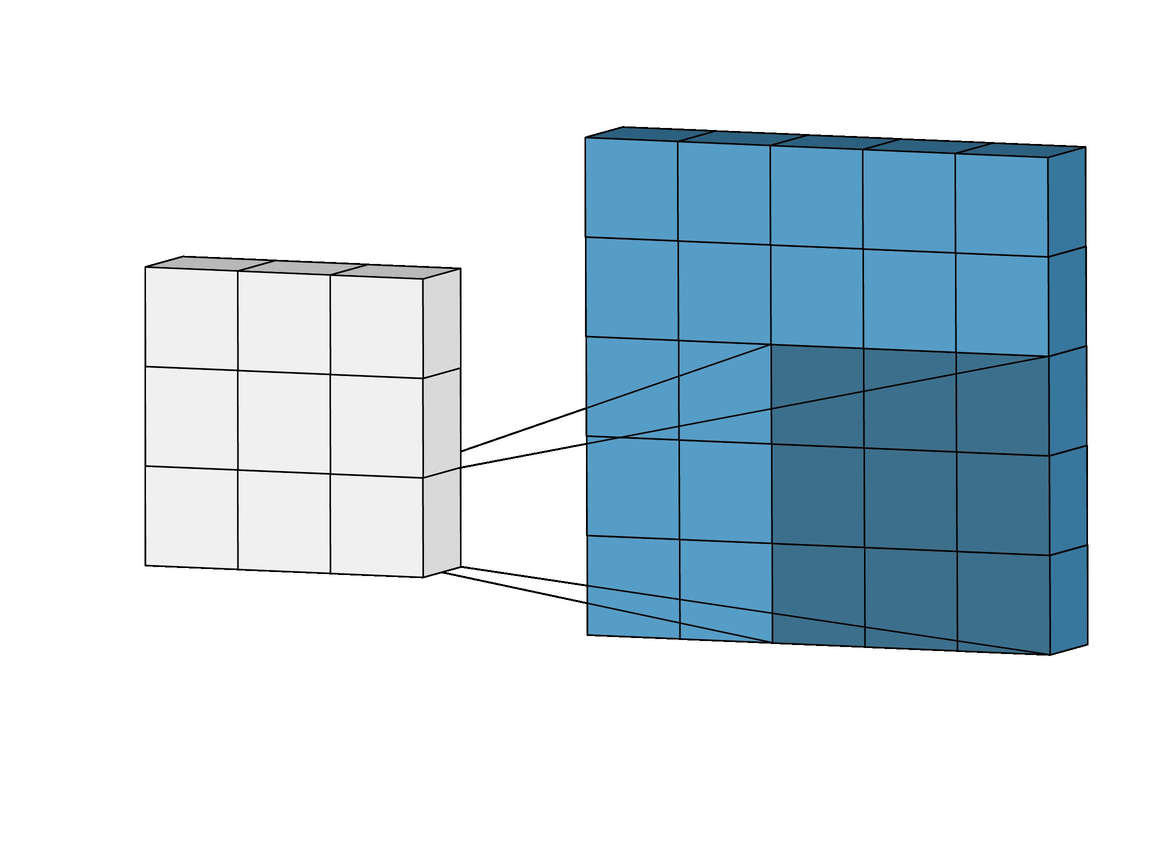
\includegraphics[width=0.8\textwidth]{figures/2d_conv/frame_8.png}
}
\end{center}
\end{column}
\end{columns}
\end{frame}

\begin{frame}{Pooling}
\begin{columns}
\begin{column}{0.5\textwidth}
\begin{itemize}
    \item Need to summarize global information more efficiently.
    \item Pooling reduces image / activation dimensions.
    \item Max-pooling or average-pooling
    \onslide<2->{
    \item You can also perform a ``strided'' convolution by jumping multiple steps.
    }
\end{itemize}
\end{column}
\begin{column}{0.5\textwidth}
\begin{center}
\mode<beamer>{
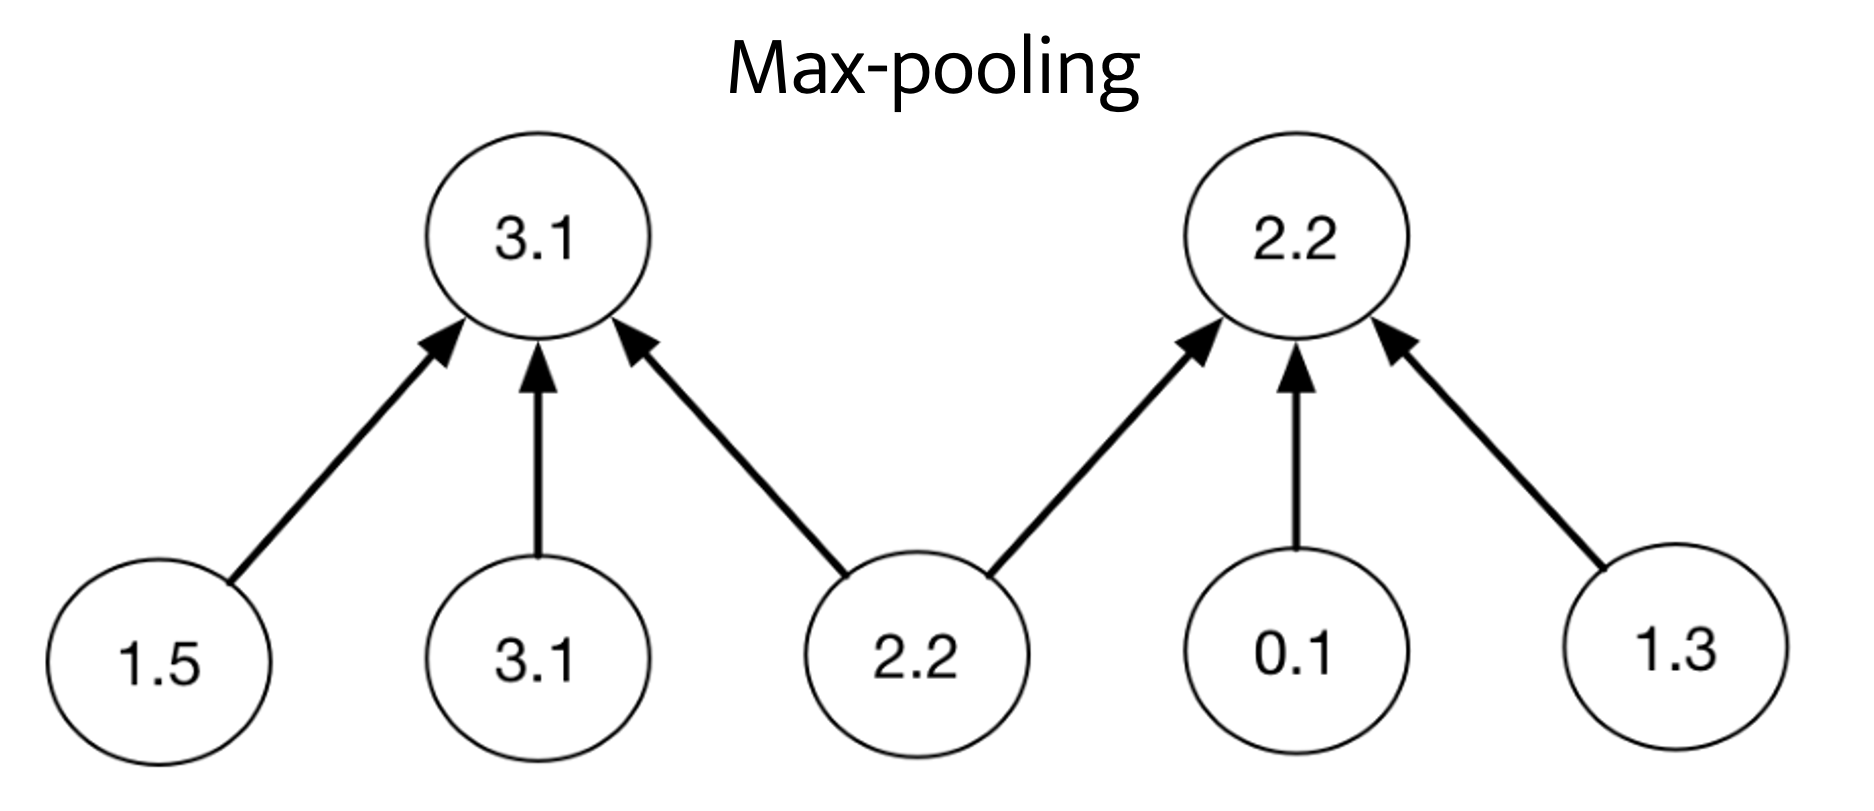
\includegraphics[width=0.8\textwidth]{figures/maxpooling.png}
\includegraphics<2>[width=0.5\textwidth]{figures/stride2_conv/frame_0.png}
\includegraphics<3>[width=0.5\textwidth]{figures/stride2_conv/frame_1.png}
\includegraphics<4>[width=0.5\textwidth]{figures/stride2_conv/frame_2.png}
\includegraphics<5>[width=0.5\textwidth]{figures/stride2_conv/frame_3.png}
}
\mode<presentation>{
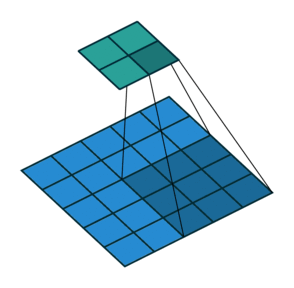
\includegraphics[width=0.5\textwidth]{figures/stride2_conv/frame_3.png}
}
\end{center}
\end{column}
\end{columns}
\end{frame}

\begin{frame}{Assembling together: LeNet}
\begin{center}
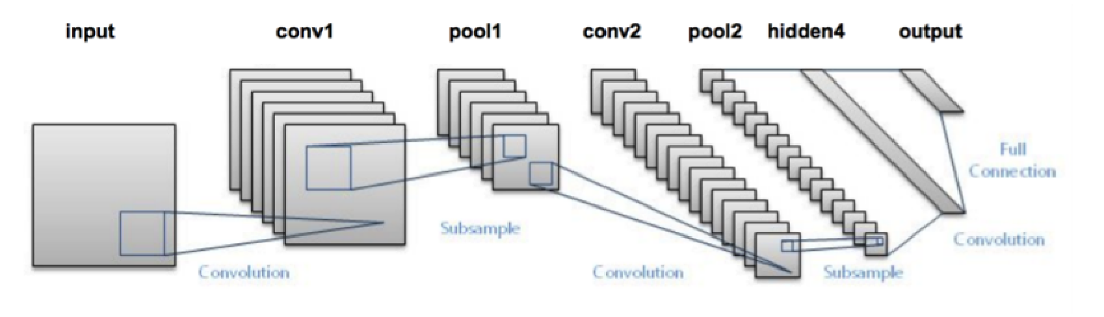
\includegraphics[width=0.8\textwidth]{figures/lenet2.png}
\end{center}
\begin{itemize}
    \item Used by USPS to read post code in the 90s.
\end{itemize}
\end{frame}

\begin{frame}{Historical development}
\begin{itemize}
    \item LeNet has worked and being put to practice in the 1990s.
    \pause
    \item Neural networks for images start to dominate in the last 10 years (starting 2012) for understanding general high resolution natural images.
    \pause
    \item During the years:
    \begin{itemize}
        \item Neural networks were difficult to work
        \item People focused on feature engineering
        \item Then apply SVM or random forest (e.g. AdaBoost face detector)
        \item What has changed?
    \end{itemize}
\end{itemize}
\end{frame}

\section{Gradient learning conditioning}
\begin{frame}{Optimization challenges}
\begin{itemize}
    \item Larger images require deeper networks (more stages of processing at different resolutions)
    \item Optimizing deeper layers of networks is not trivial.
    \item Loss often stalls or blows up.
    \pause
    \item Why?
    \pause
    \begin{itemize}
        \item Backpropagation: multiplying the Jacobian $\frac{\partial y}{\partial x}$ by each layer.
        \item If the maximum singular value of each layer of Jacobian is less than 1: then the gradient will converge to 0 with more layers.
        \item If the greater than 1: then the gradient will explode with more layers.
        \item The bottom (input) layer may get 0 or infinite gradients.
    \end{itemize}
\end{itemize}
\end{frame}

\begin{frame}{Weight initialization}
\begin{itemize}
    \item<+-> Even with a few layers (>3), optimization is still hard.
    \item<+-> If weight initialization is bad (too small or too big), then optimization is hard to kick off.
    \item<+-> Consider the distribution of whole dataset in the activation space.
    % \item Pre-activation: $z=Wx$; Post-activation: $h=f(z)$
    \begin{itemize}
        % \item The mean of the pre-activations should be zero.
        \item Intuition: upon initialization, the variance of the activations should stay the same across every layer.
    \end{itemize}
\end{itemize}
\end{frame}

\begin{frame}{Kaiming Initialization}
\begin{itemize}
    \item Suppose each neuron and weight connection are sampling from a random distribution.
    \pause
    \item At $l$-th layer, $Var[z_l] = n_l Var[w_l x_l]$ ($n_l$ = num. input neurons to $l$-th layer)
    \pause
    \item If we suppose that ReLU is used as the activation, and $w_l$ is symmetric and zero-mean, $x_{l+1} = \frac{1}{2} Var[z_{l}]$.
    \pause
    \item Putting altogether, $x_{l+1} = \frac{1}{2} n_l Var[w_{l}] Var[x_l]$.
    \pause
    \item To make the variance constant, we need $\frac{1}{2} n_l Var[w_{l}] = 1$, $Std[w_{l}] = \sqrt{2/n_l}$\footnote{
    \tiny He et al. Delving Deep into Rectifiers: Surpassing Human-Level Performance on ImageNet. ICCV, 2015.}.
\end{itemize}
\end{frame}

\begin{frame}{Activation functions}
\begin{itemize}
    \item ReLU was proposed in 2009-2010\footnote{\tiny Jarrett et al. What is the Best Multi-Stage Architecture for Object Recognition? ICCV, 2009.}\footnote{\tiny Nair \& Hinton/ Rectified Linear Units Improve Restricted Boltzmann Machines. ICML, 2010.}, and was successfully used in AlexNet in 2012\footnote{\tiny Krizhevsky et al. 
ImageNet Classification with Deep Convolutional Neural Networks. NIPS, 2012.}.
    \item Address the vanishing gradient issue in activations, comparing to sigmoid or tanh.
    % \item More variants of activation function in the past decade.
\end{itemize}
\begin{center}
    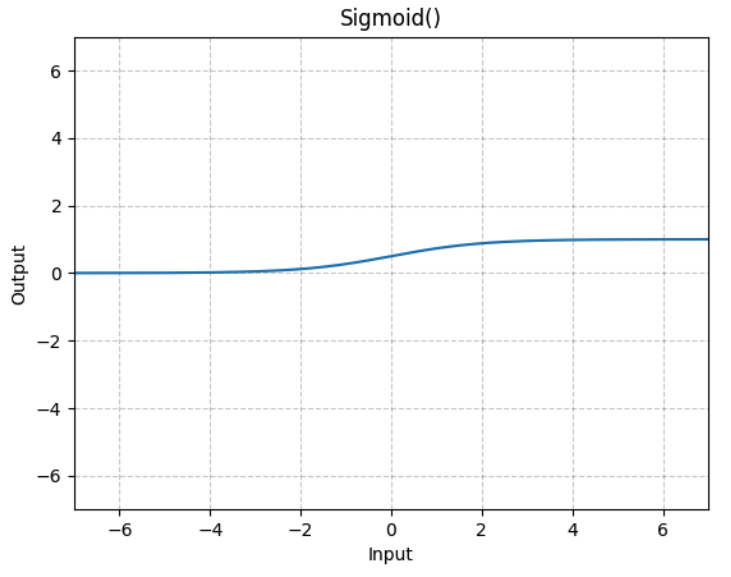
\includegraphics[width=0.17\textwidth]{figures/sigmoid.png}
    \quad
    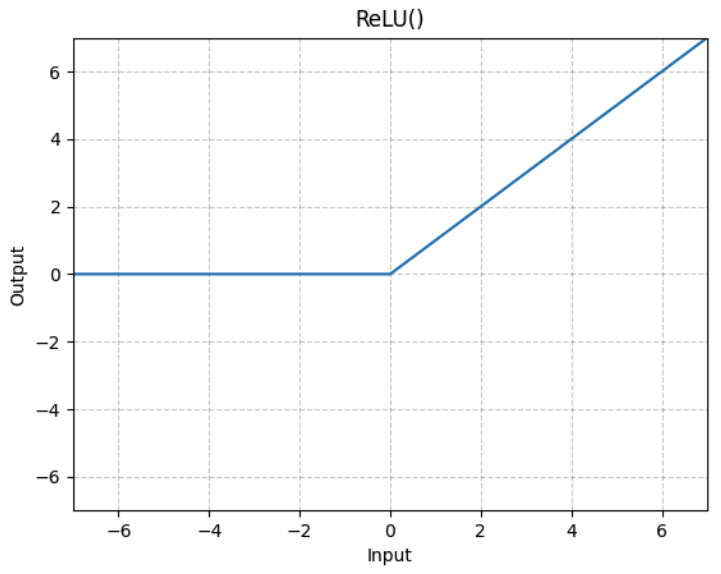
\includegraphics[width=0.17\textwidth]{figures/relu.png}
    \quad
    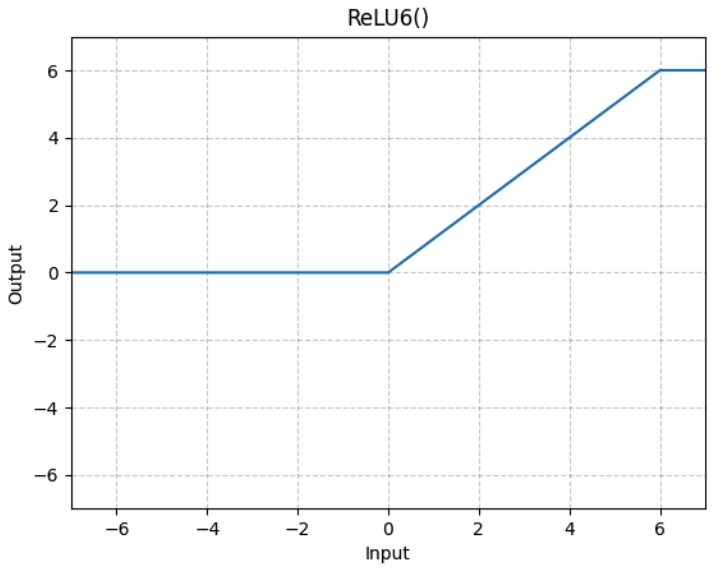
\includegraphics[width=0.17\textwidth]{figures/relu6.png}

    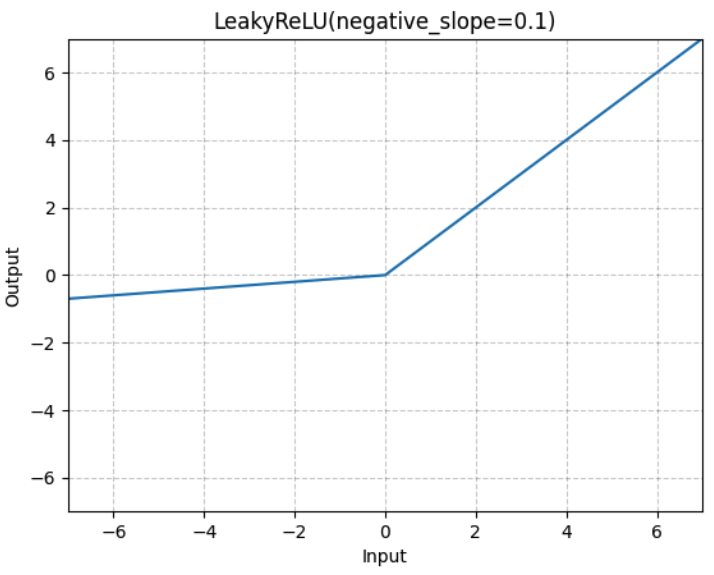
\includegraphics[width=0.17\textwidth]{figures/leaky_relu.png}
    \quad
    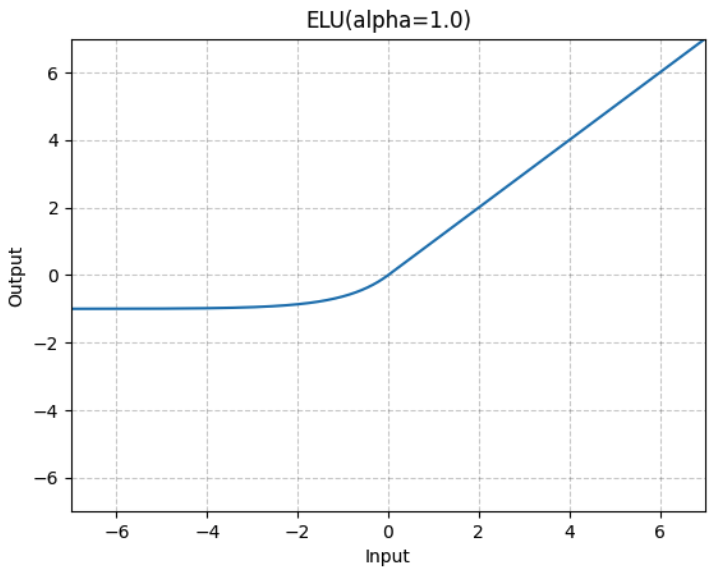
\includegraphics[width=0.17\textwidth]{figures/elu.png}
    \quad
    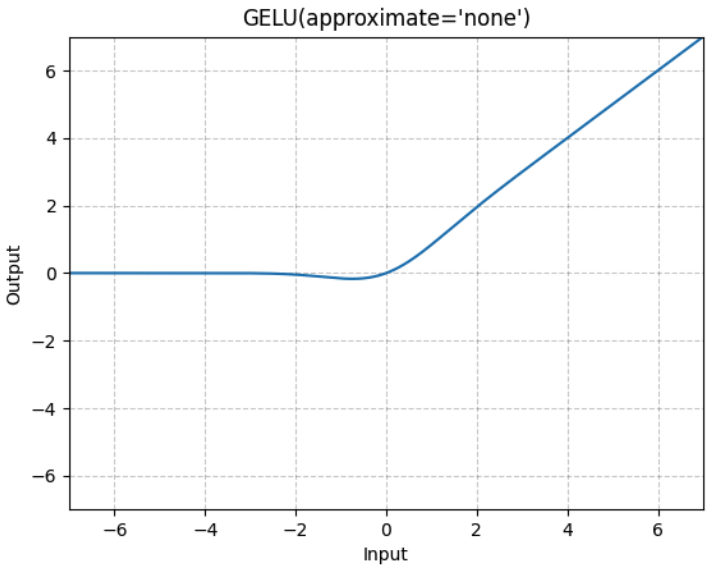
\includegraphics[width=0.17\textwidth]{figures/gelu.png}
\end{center}
\end{frame}

\begin{frame}{SGD Learning Rate}
  \begin{itemize}
    \item In stochastic training, the learning rate also influences the \alert{fluctuations} due to the stochasticity of the gradients.
    \item Typical strategy:
      \begin{itemize}
        \item Use a large learning rate early in training so you can get close to the optimum.
        \item Gradually decay the learning rate to reduce the fluctuations.
      \end{itemize}
  \end{itemize}
\end{frame}

\begin{frame}{Learning Rate Decay}
    \begin{itemize}
      \item We also need to be aware about the impact of learning rate due to the stochasticity.
    \end{itemize}
    \begin{center}
      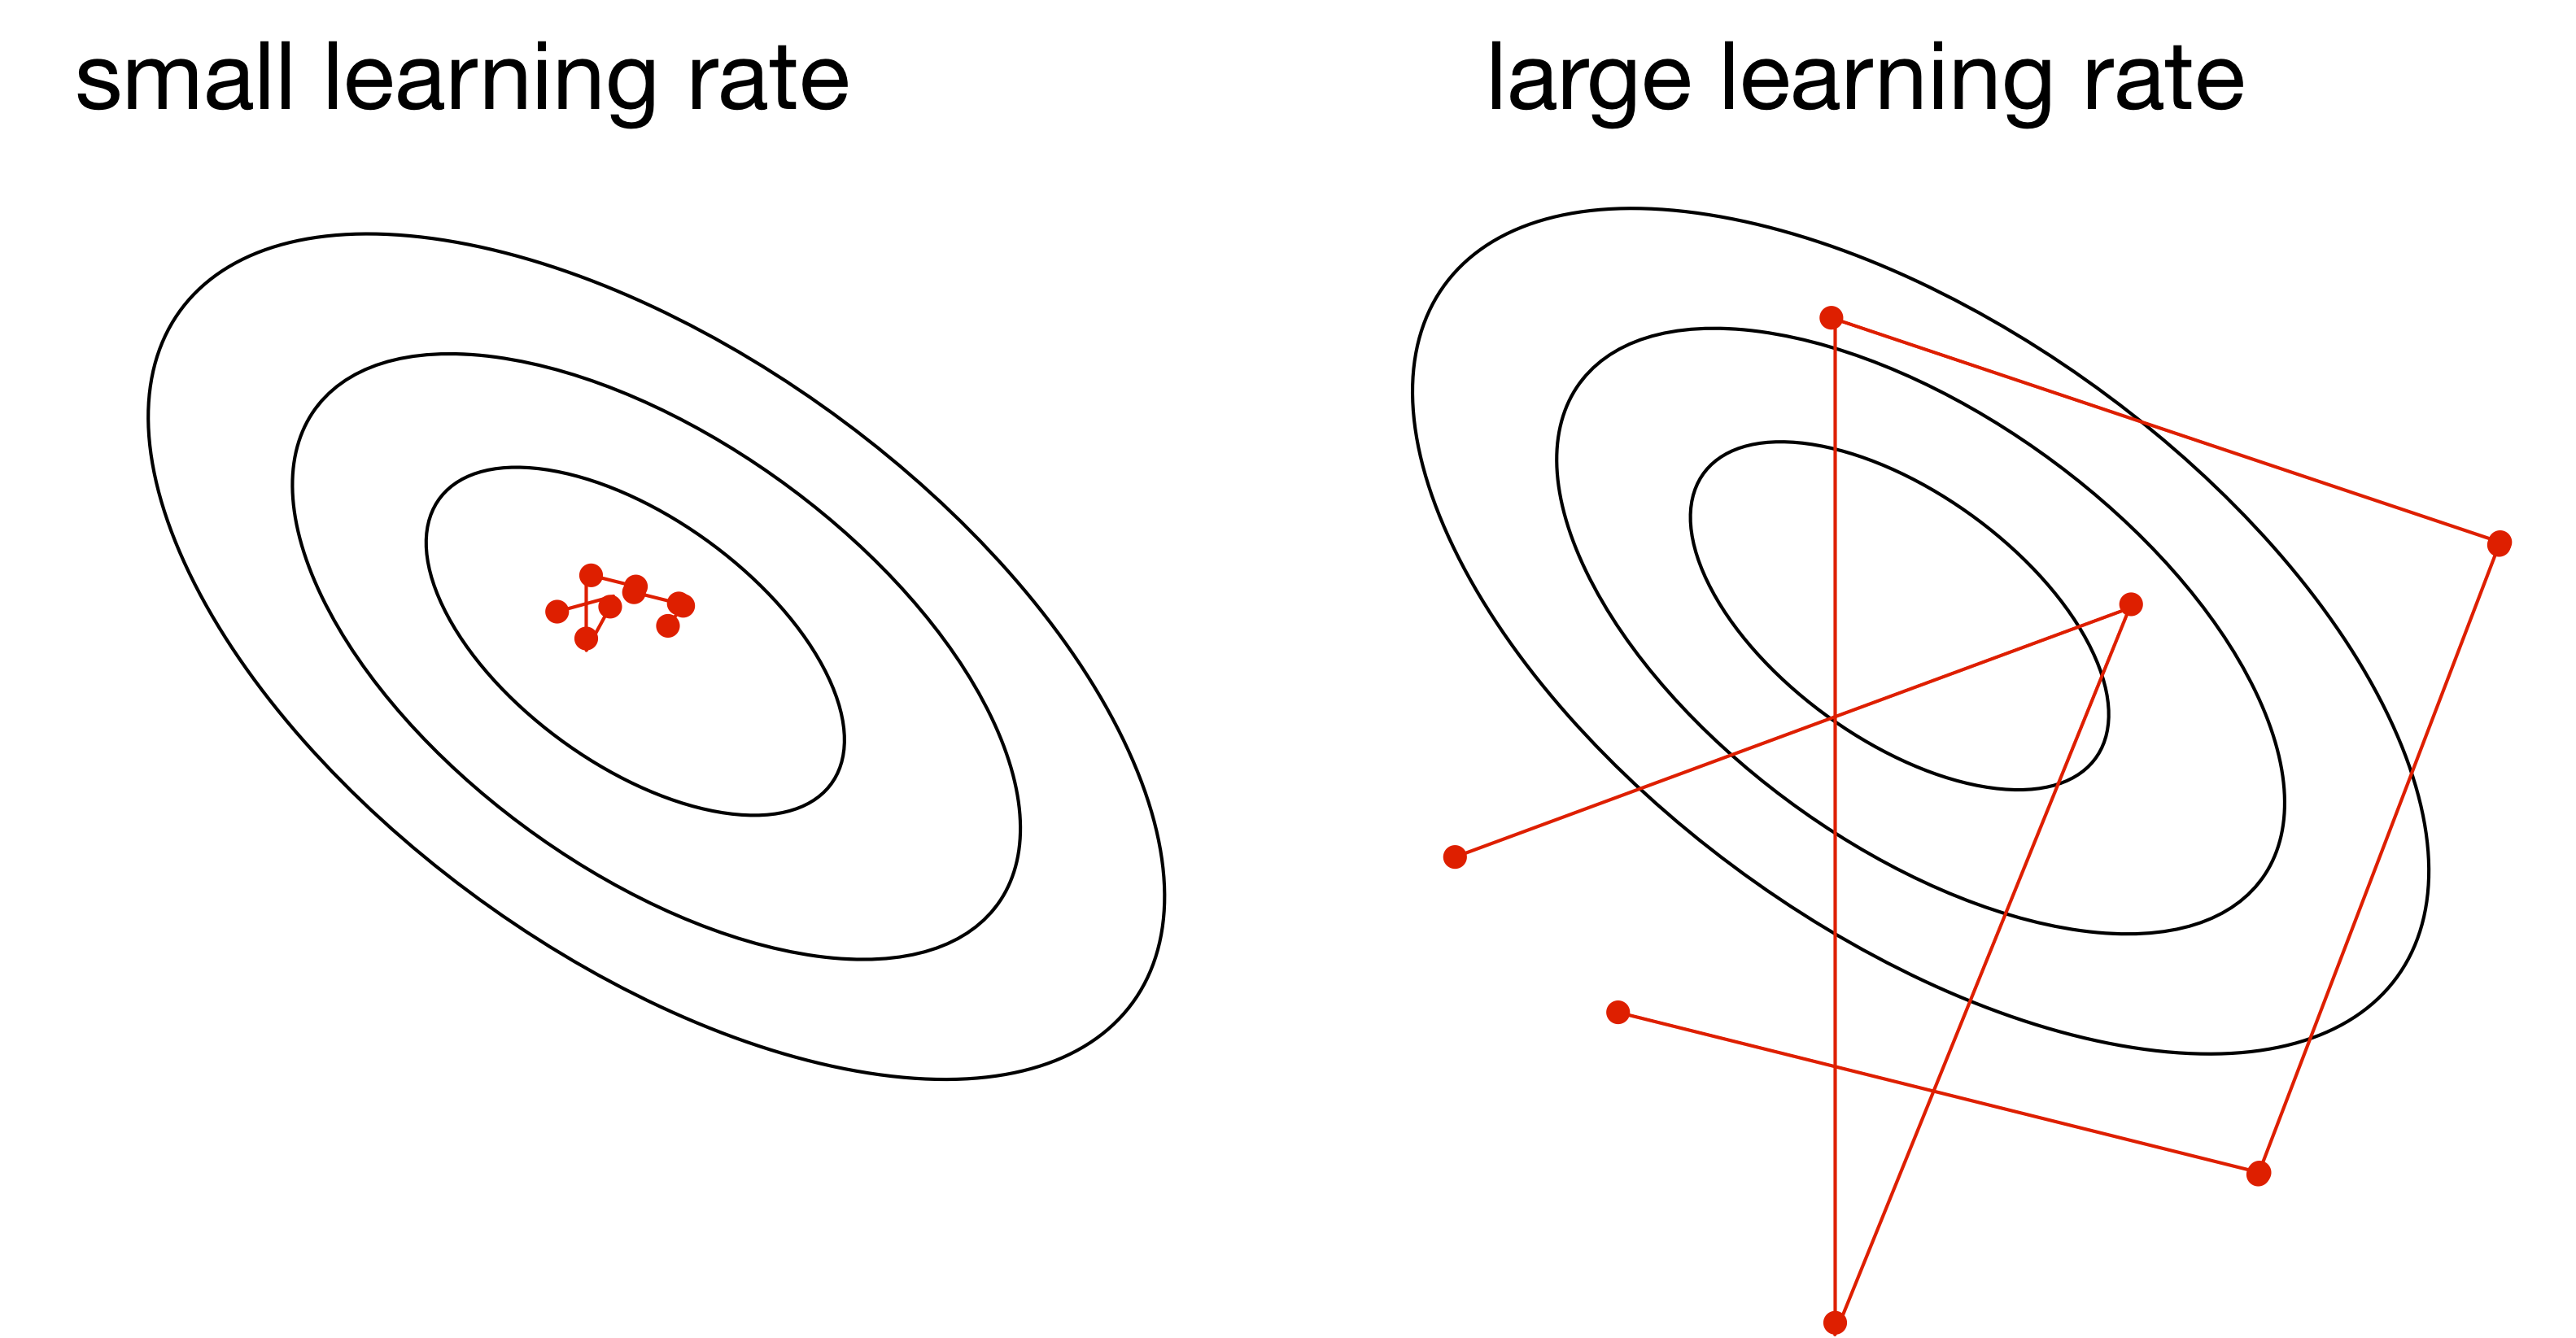
\includegraphics[width=0.3\textwidth]{figures/fluctuations.png}
    \end{center}
    \begin{center}
      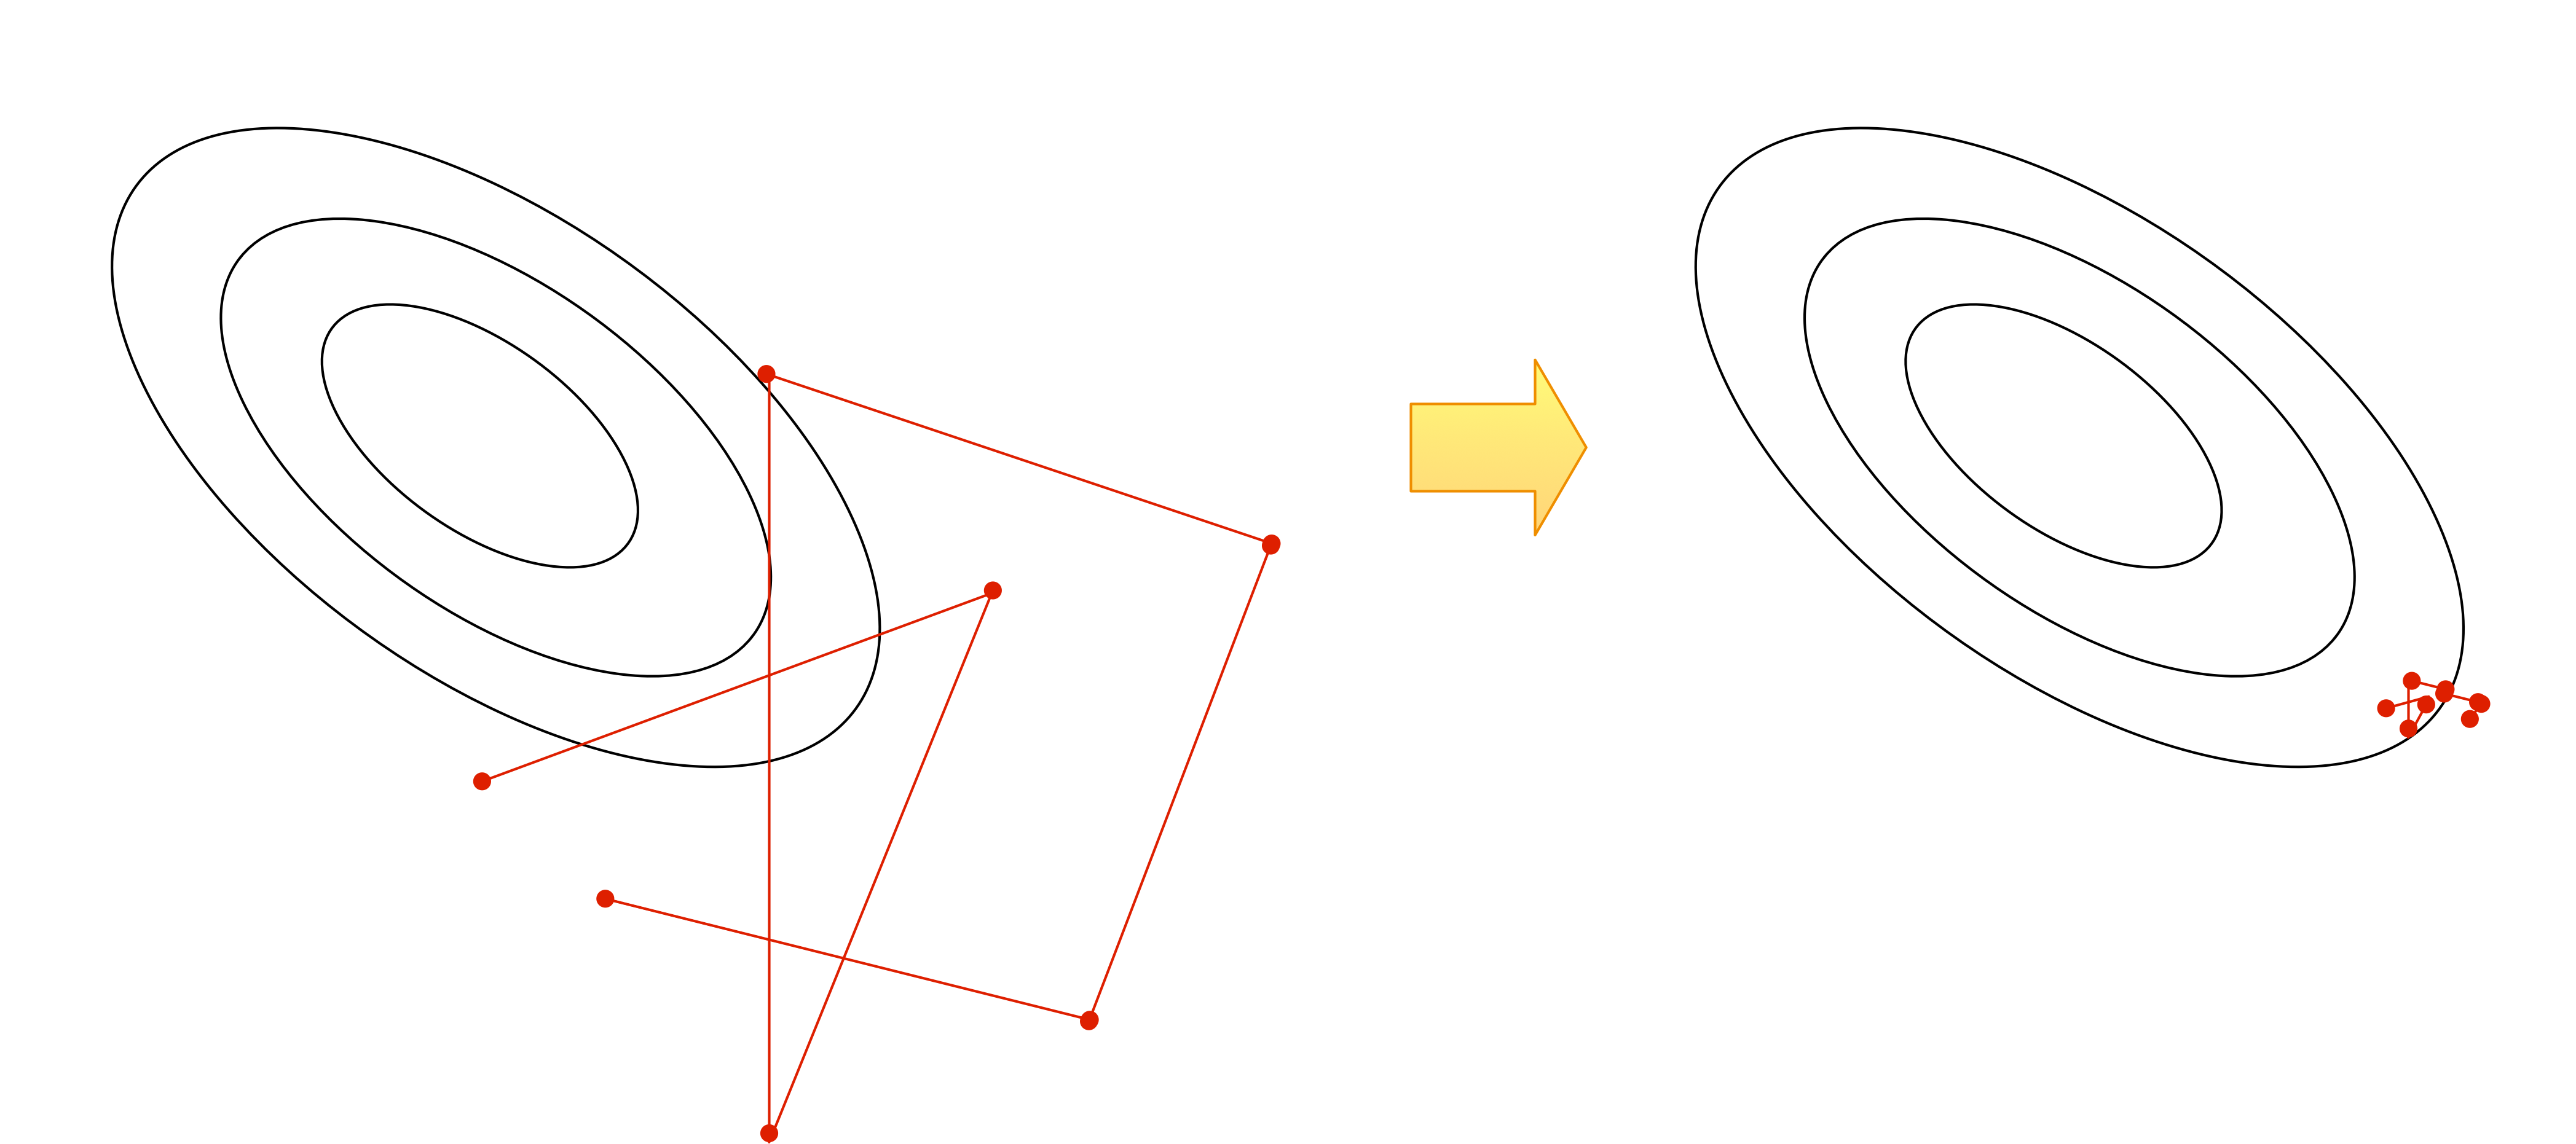
\includegraphics[width=0.25\linewidth]{figures/premature_lr_decay.png}
      \hspace{0.05 \linewidth}
      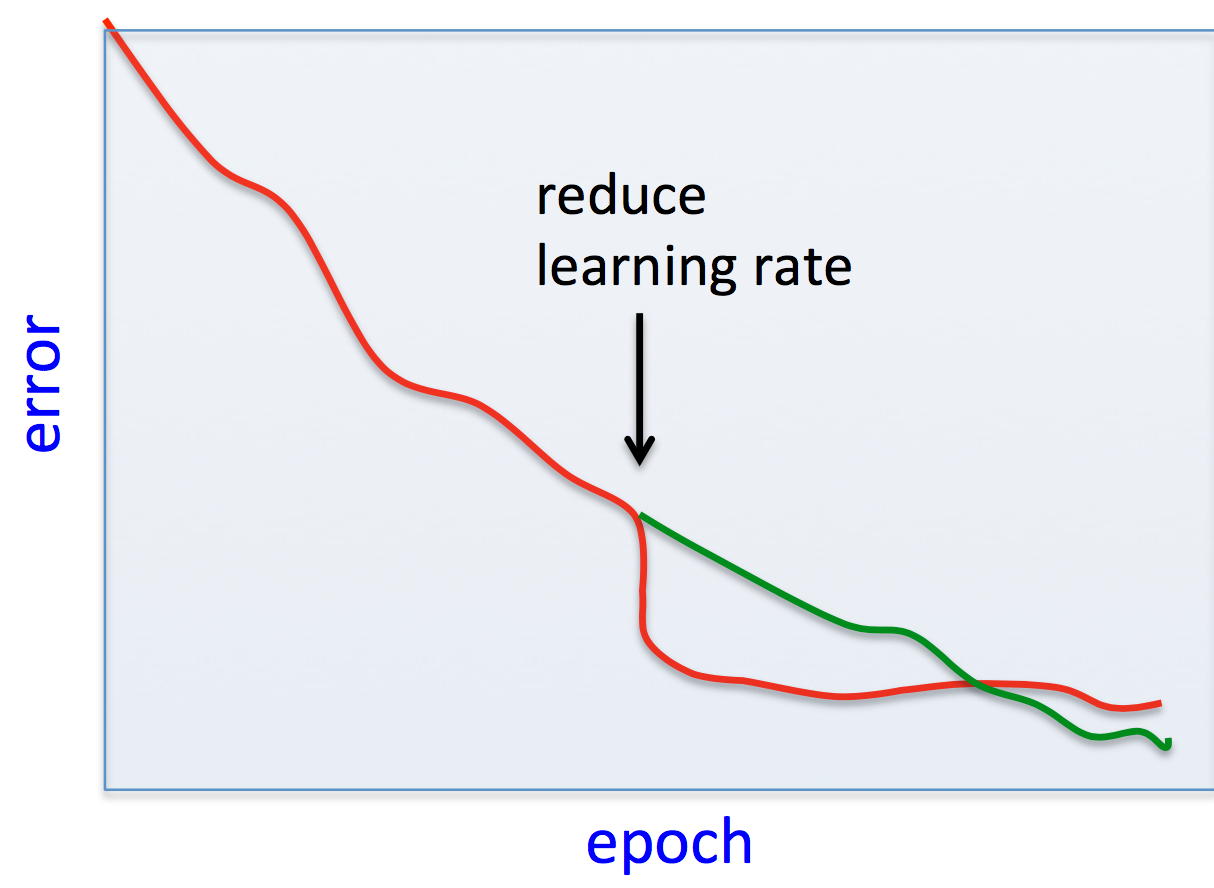
\includegraphics[width=0.25\linewidth]{figures/sgd_learning_curves.png}
    \end{center}
\end{frame}

\begin{frame}{RMSprop and Adam}
  \begin{itemize}
  \item Recall: SGD takes large steps in directions of high curvature and small steps in directions of low curvature.
  \item<+-> \alert{RMSprop} is a variant of SGD which rescales each coordinate of the gradient to have norm 1 on average. It does this by keeping an exponential moving average $s_j$ of the squared gradients.
  \item<+-> The following update is applied to each coordinate $j$ independently:
    \begin{align*}
      s_j &\gets (1-\gamma) s_j + \gamma [\tfrac{\partial L}{\partial \theta_j}]^2 \\
      \theta_j &\gets \theta_j - \frac{\alpha}{\sqrt{s_j + \epsilon}} \frac{\partial L}{\partial \theta_j}
    \end{align*}
  % \item Both optimizers are included in TensorFlow, Pytorch, etc.
  \end{itemize}
  % \notenew{
  % \begin{itemize}
  %   \item Draw a skewed axis-aligned quadratic.
  %   \item If the eigenvectors of the Hessian are axis-aligned (dubious assumption), then RMSprop can correct for the curvature. In practice, it typically works slightly better than SGD.
  % \end{itemize}
  % }
\end{frame}

\begin{frame}{Adam optimizer}
\begin{columns}
\begin{column}{0.6\textwidth}
\begin{itemize}
  \item<+-> \alert{Adam} = RMSprop + momentum = Adaptive Momentum estimation
  \item<1-> Smoother estimate of the average gradient and gradient norm.
  \item<+-> $m_t$: exponential moving average of gradient.
  \item<2-> $v_t$: exponential moving average of gradient squared.
  \item<2-> $\hat{m}_t$, $\hat{v}_t$: Bias correction.
  \item<2-> $\theta_t \leftarrow \theta_{t-1} - \alpha \hat{m}_t / (\sqrt{\hat{v_t}} + \epsilon)$
  \item<2-> The ``default'' optimizer for modern networks.
\end{itemize}
\end{column}
\begin{column}{0.38\textwidth}
\begin{center}
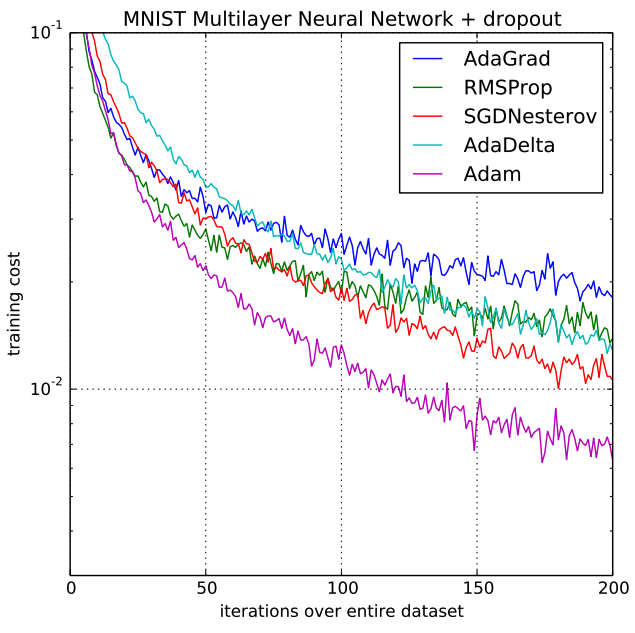
\includegraphics[width=0.8\textwidth]{figures/adam.png}
\end{center}
\end{column}
\end{columns}
\end{frame}

\begin{frame}{Normalization}
% \begin{columns}
% \begin{column}{0.6\textwidth}
\begin{itemize}
    \item<+-> Weight initialization is tricky, and there is no guarantee that the distribution of activations will stay the same over the learning process.
    \item<1-> What if the weights keep grow bigger and activation may explode?
    \item<+-> We can ``normalize'' the activations.
    \item<2-> The idea is to control the activation within a normal range: zero-mean, uni-variance.
\end{itemize}
% \end{column}
% \begin{column}{0.38\textwidth}
% \begin{center}
% 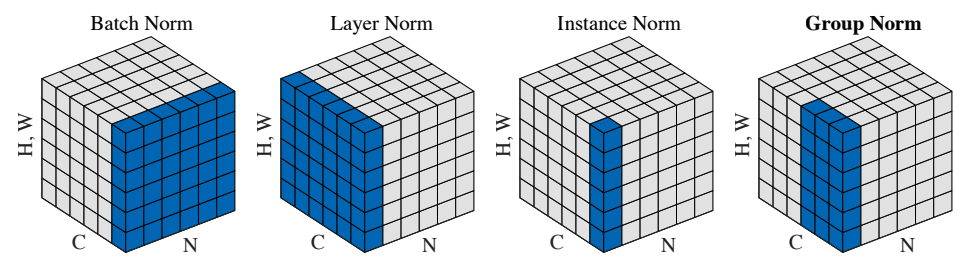
\includegraphics[width=0.8\textwidth]{figures/normalization.png}
% \end{center}
% \end{column}
% \end{columns}
\end{frame}

\begin{frame}{Batch Normalization (BN)}

\begin{columns}
\begin{column}{0.6\textwidth}
\begin{itemize}
    % \item What is the population to normalize it from?
    % \item Training image distribution -> activation distribution
    \item<+-> In CNNs, neurons across different spatial locations are also samples of the same feature channel.
    \item<+-> Batch norm: Normalize across N H W dimensions, leaving C channels.
    \item<+-> $\tilde{x} = \gamma \frac{x - \mu}{\sigma} + \beta$
    \item<3-> $\gamma, \beta$: learnable parameters. $\mu, \sigma$: statistics from the training batch.
    \item<+-> Test time: using the mean and variance from the entire training set.
\end{itemize}
\end{column}

\begin{column}{0.38\textwidth}
\begin{center}
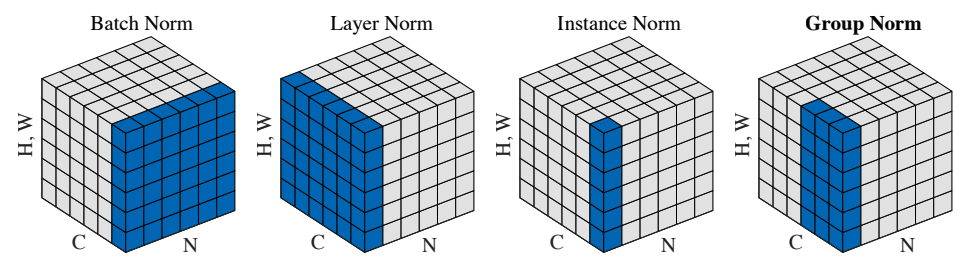
\includegraphics[width=0.7\textwidth,trim={0 0 25.5cm 0},clip]{figures/normalization.png}
\end{center}
\end{column}
\end{columns}

\end{frame}

\begin{frame}{BN Alternatives}
\begin{itemize}
    \item Need a considerable batch size to estimate mean and variance correctly.
    \item Training is different from testing.
    \item Alternatives consider the C channel dimension instead of N batch dimension.
    % \item No longer estimating the distribution from training samples.
\end{itemize}
\begin{center}
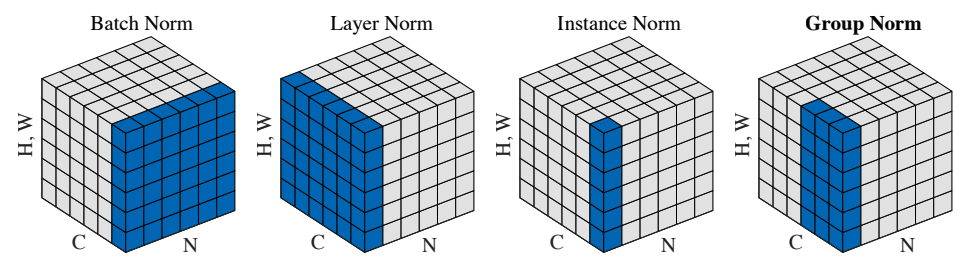
\includegraphics[width=0.6\textwidth,trim={10cm 0 0 0},clip]{figures/normalization.png}
\footnote{\tiny Wu and He. Group normalization. ECCV 2018.}
\end{center}
\end{frame}

\begin{frame}{Going Deeper}
\begin{itemize}
    \item The progress of normalization allowed us to train even deeper networks.
    \item The networks are no longer too sensitive with initialization.
    \item<+-> But the best networks were still around 20 layers and deeper results in worse performance.
\end{itemize}
\begin{center}
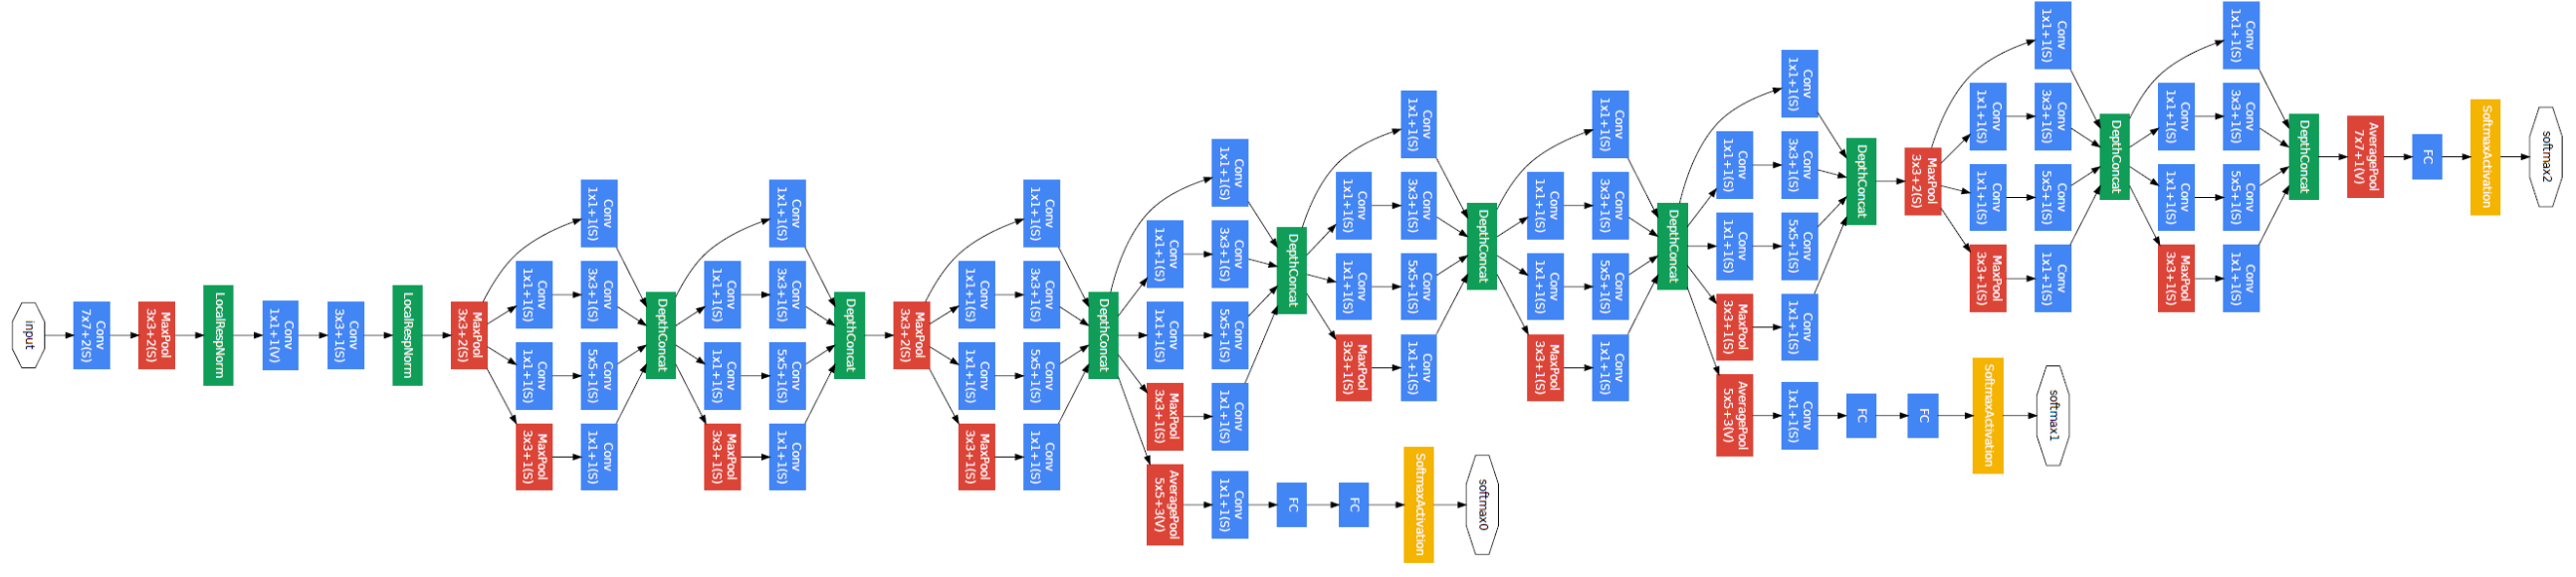
\includegraphics[width=0.6\textwidth]{figures/googlenet.png}
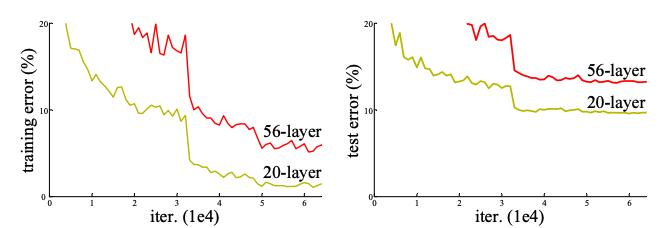
\includegraphics[width=0.35\textwidth]{figures/20layer.png}
\end{center}
\end{frame}

\begin{frame}{Residual Networks (ResNet)}

\begin{itemize}
    \item Recall in gradient boosting, we are iteratively adding a function to the model to expand the capacity.
    \item Residual connection: Skip connection to prevent gradient vanishing.\footnote{\tiny He et al. Deep Residual Learning for Image Recognition. CVPR 2016.}
    % \item A simple ``addition'' operation on the activation.
\end{itemize}

\begin{center}
% 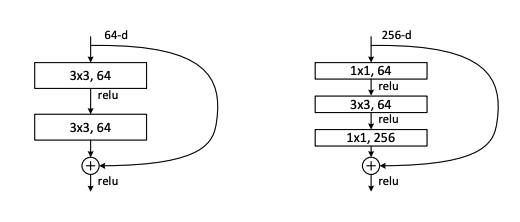
\includegraphics[width=0.75\textwidth]{figures/residual_connect.png}
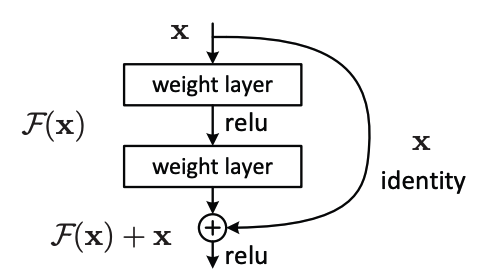
\includegraphics[width=0.5\textwidth]{figures/resnet.png}
\end{center}

\end{frame}

\begin{frame}{ResNet Success}
\begin{itemize}
    \item Now able to train over 100 layers.
    \item One of the most important network design choices in the past decade.
    \item Prevalent in almost all network architectures, including Transformers.
    \pause
    \item Loss landscape view: Skip connections makes loss smoother -> easier to optimize \footnote{\tiny Li et al. Visualizing the Loss Landscape of Neural Nets. NIPS 2018.}.
\end{itemize}
\begin{center}
% 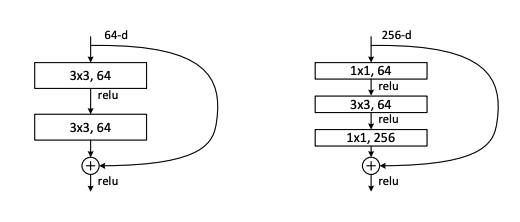
\includegraphics[width=0.75\textwidth]{figures/residual_connect.png}
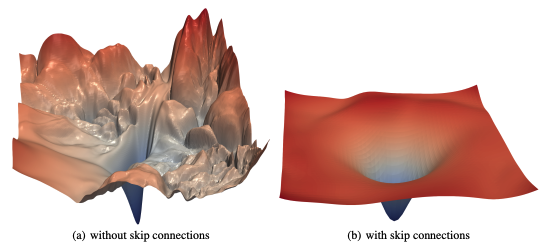
\includegraphics[width=0.5\textwidth]{figures/resnetlandscape.png}
\end{center}
\end{frame}

\begin{frame}{Dropout\footnote{\tiny Srivastava et al. A Simple Way to Prevent Neural Networks from Overfitting. JMLR, 2014.}
}
\begin{itemize}
    \item Want to reduce overfitting in neural networks.
    \item Stochastically turning off neurons in propagation.
    \onslide<2->{
    \item Training to preserve redundancy.
    \item Test time: multiplying activations with probability. Model ensembling effect.
    }
\end{itemize}
\begin{center}
\onslide<1->{
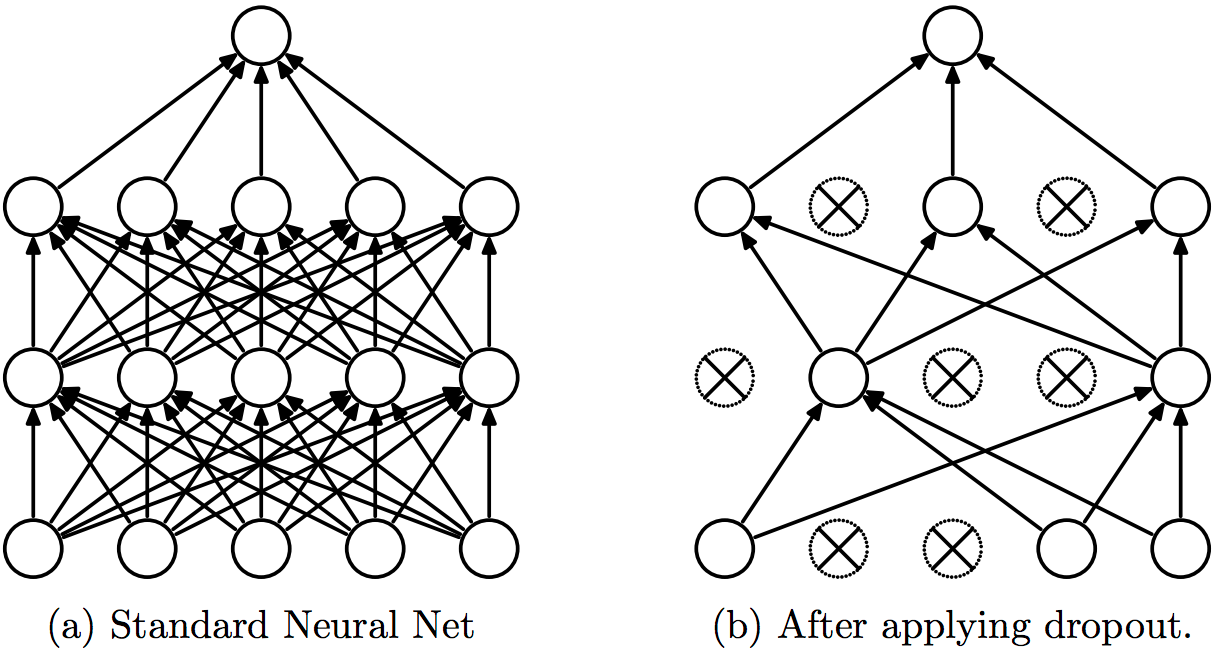
\includegraphics[width=0.4\textwidth]{figures/dropout.png}
}
\end{center}

\end{frame}

\begin{frame}{GELU\footnote{\tiny Hendrycks \& Gimpel. Gaussian Error Linear Unit (GELU). CoRR abs/1606.08415, 2016.}}
\begin{columns}
\begin{column}{0.49\textwidth}
\begin{itemize}
    \item Gaussian Error Linear Unit - A smoother activation function. 
    \item Motivated by Dropout.
    \onslide<2->{
    \item $f(x) = \mathbb{E}[x \cdot m].$
    }
    \onslide<3->{
    \item $m \sim Bernoulli(\Phi(x)).$
    \item $\Phi(x) = P(X \le x).$
    \item $X \sim \mathcal{N}(0,1).$
    }
\end{itemize}
\end{column}
\begin{column}{0.49\textwidth}
\begin{center}
    \onslide<1->{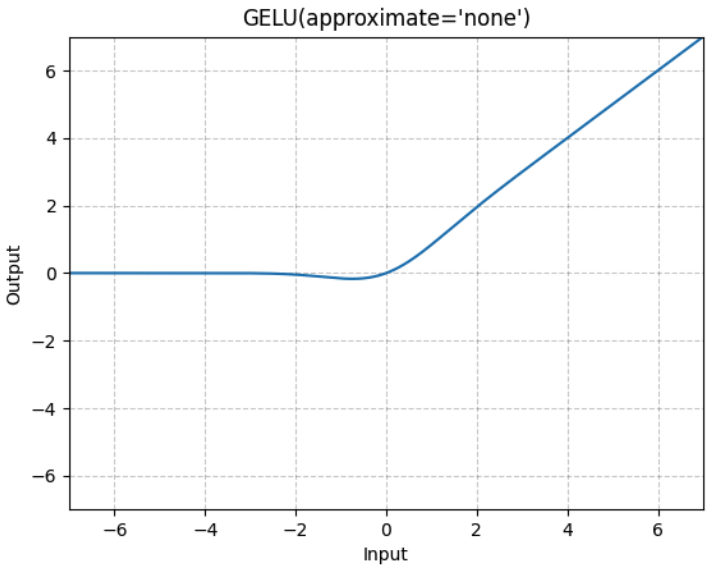
\includegraphics[width=0.8\textwidth]{figures/gelu.png}}
\end{center}
\end{column}
\end{columns}
\end{frame}

\begin{frame}{Data augmentation}
\begin{columns}
\begin{column}{0.4\textwidth}
\begin{itemize}
    \item Leverage the invariances of images
    \item Create more data points for free
    \begin{itemize}
    \item<2->Random cropping
    \item<3->Left+right flipping
    \item<4->Random color jittering
    \item<5->Random blurring
    \item<6->Affine warping
    \item<6->Etc.
    \end{itemize}
\end{itemize}
\end{column}
\begin{column}{0.59\textwidth}
\onslide<1->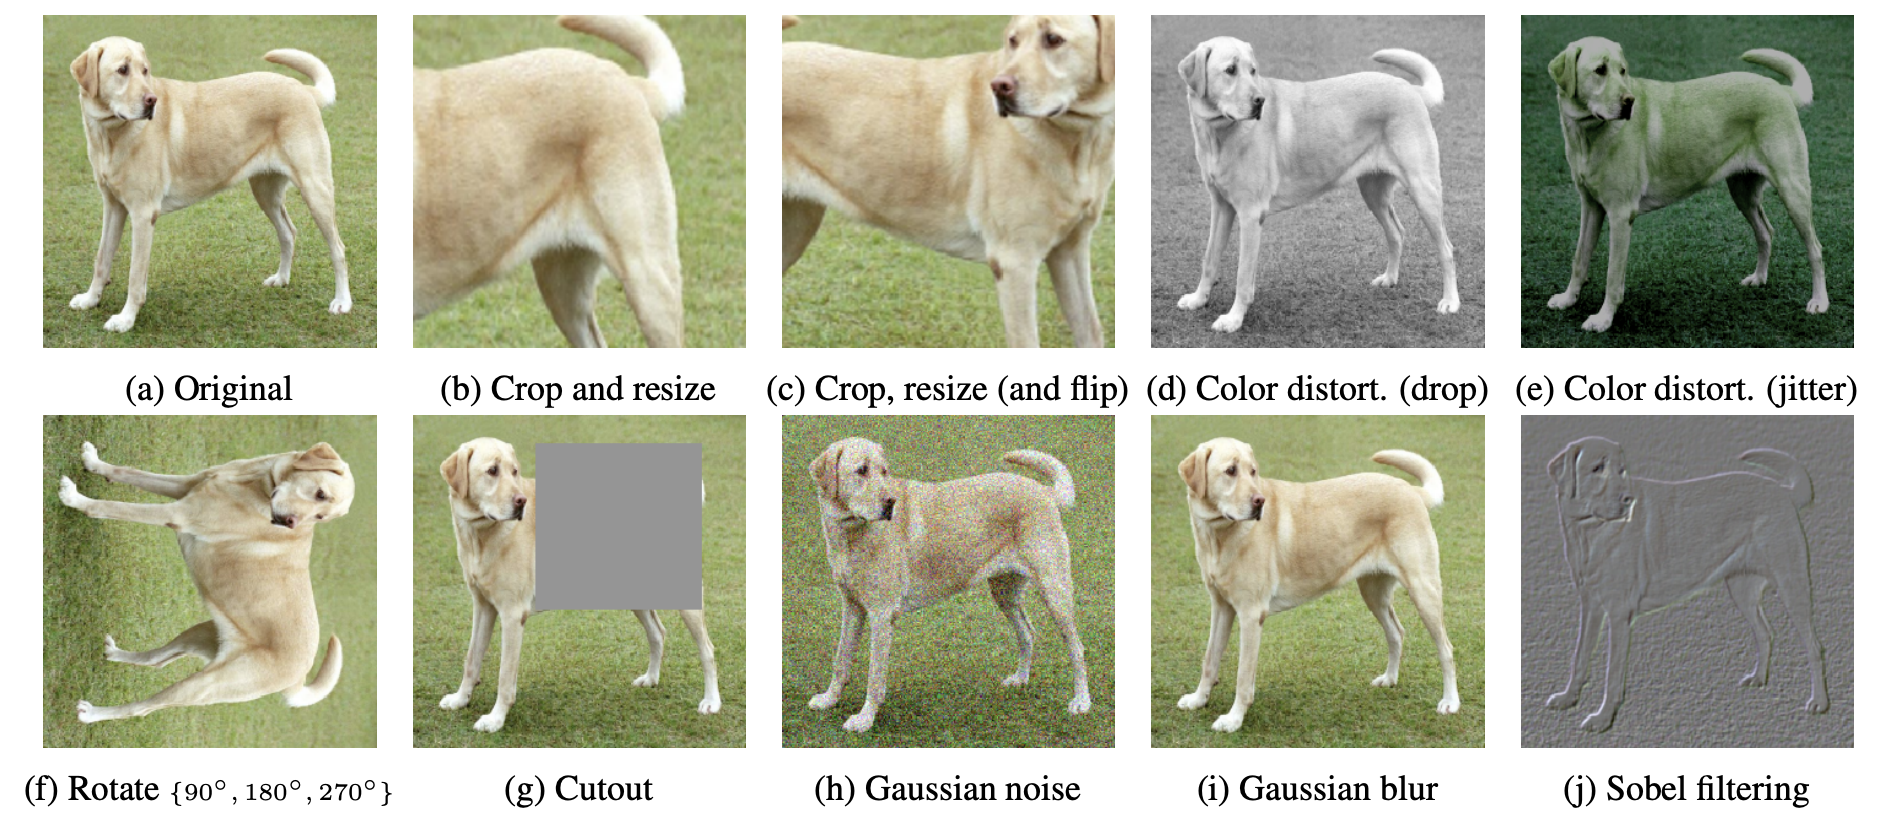
\includegraphics[width=0.9\textwidth]{figures/data_aug.png}
\end{column}
\end{columns}
    \small{Image credit}\footnote{\tiny Chen et al. A Simple Framework for Contrastive Learning of Visual Representations. ICML 2020.}
\end{frame}

\section{Language and sequential signals}
\begin{frame}{What about natural language}
\begin{itemize}
    \item<+-> Neural networks are great for dealing with naturalistic and unstructured signals.
     % such as images, sound, language, where there are no good manual feature extractors.
    \item<+-> Past lectures: Feature functions in structured models, but still primitive.
    \item<+-> Design neural networks to accomodate sequential signals such as language.
\end{itemize}
\begin{center}
\onslide<1->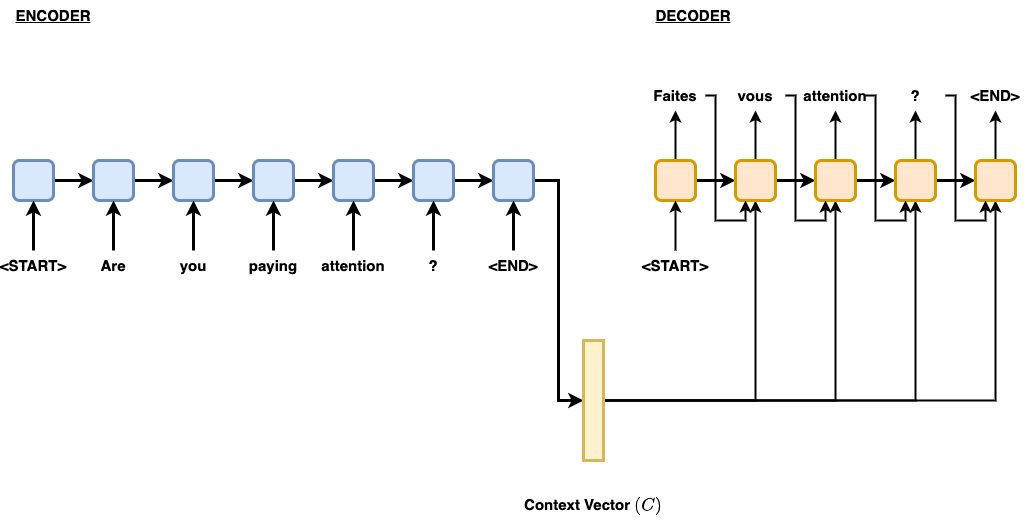
\includegraphics[width=0.7\textwidth,trim={0 0 0 3cm},clip]{figures/neural-machine-translation.png}
\end{center}
\end{frame}

\begin{frame}{Word embeddings}
\begin{itemize}
    \item<+-> Neural networks are best dealing with real valued vectors.
    \item<+-> Need to convert words (discrete) into vectors (continuous).
    \item<+-> A large matrix of $V \times D$. V = vocab size, D = network embedding size.
\end{itemize}
\begin{center}
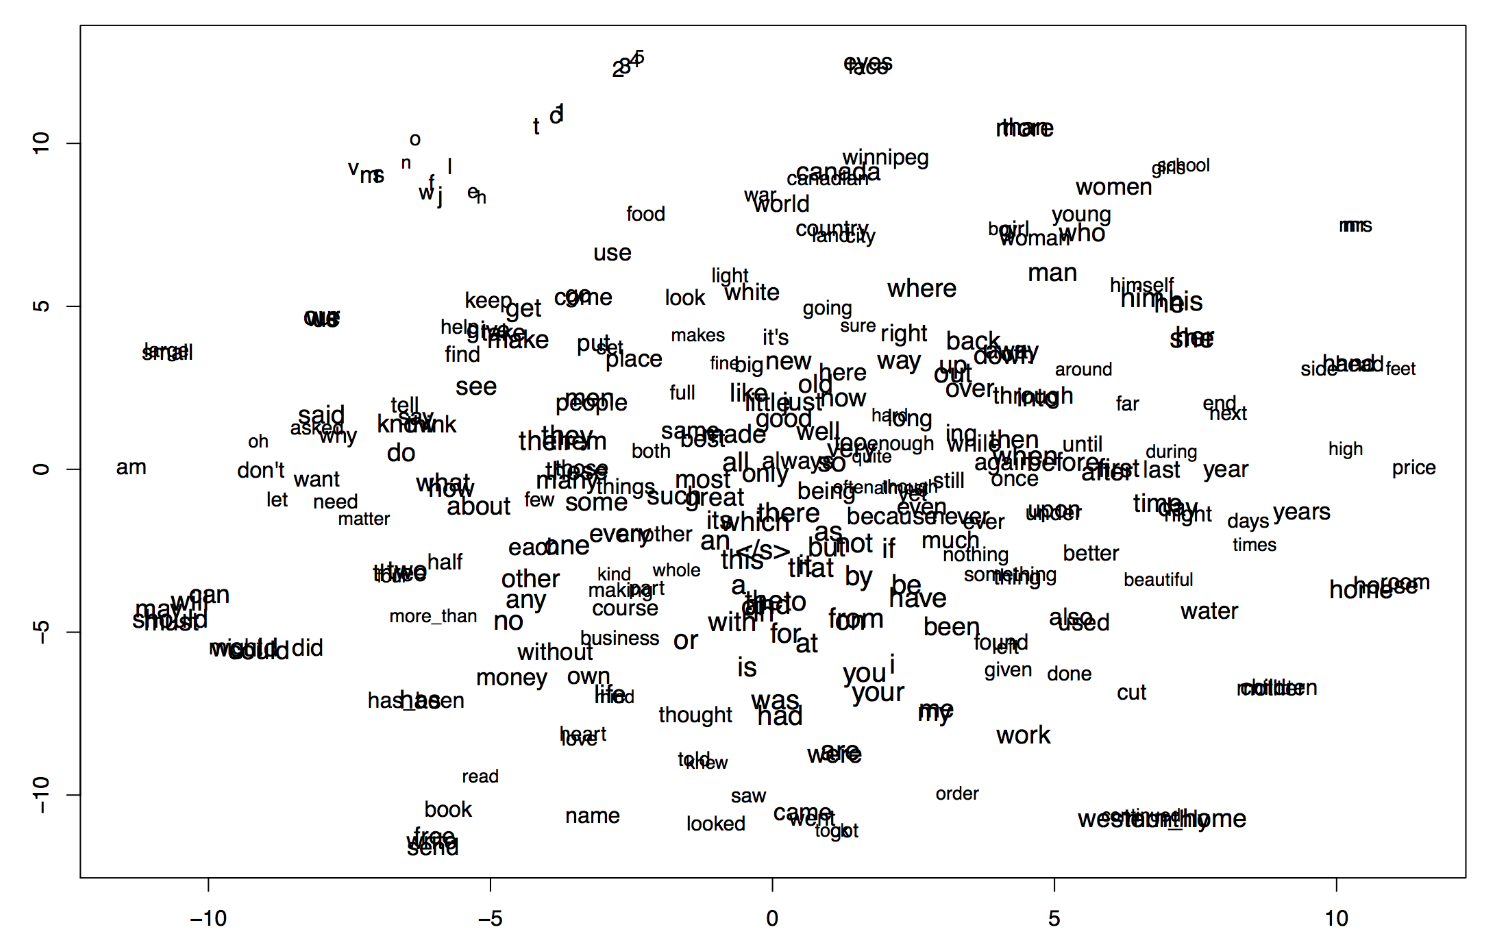
\includegraphics[width=0.4\textwidth]{figures/word_embedding.png}\footnote{\tiny \url{https://aelang.github.io/word-embeddings.html}}
\end{center}
\end{frame}

\begin{frame}{Convolutional vs. recurrent networks}
\begin{itemize}
    \item<+-> Recall in images we used the convolution operation.
    \item<1-> We can also use the idea of convolution for temporal signals.
    \item<+-> Another alternative is to use a type of network called recurrent networks.
    \item<2-> Two inputs: $\mathbf{x}_t$ is the current input, and $\mathbf{h}_t$ is the historical hidden state.
    \item<+-> We can unroll the computation graph into a direct acyclic graph (DAG).
\end{itemize}
\begin{center}
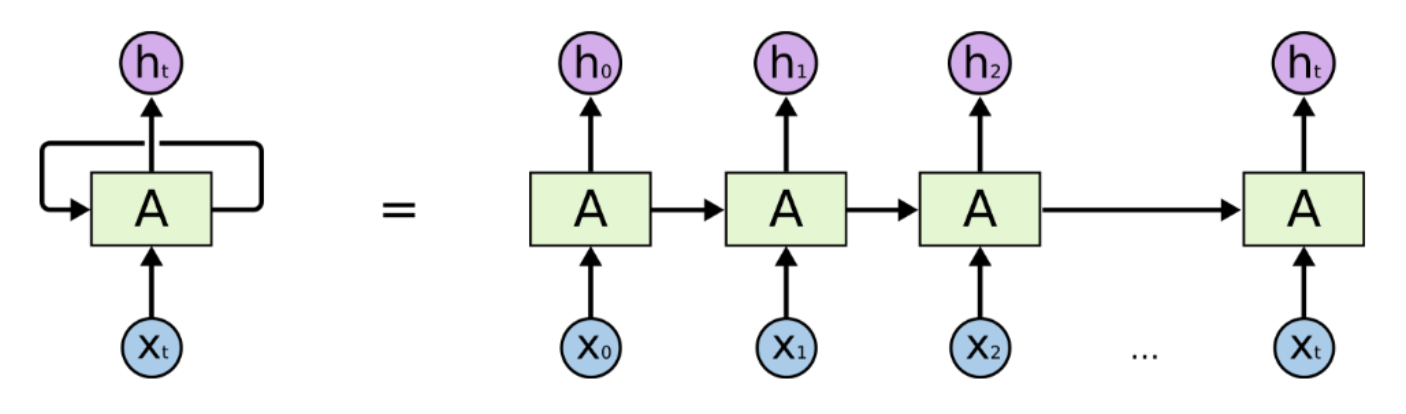
\includegraphics[width=0.7\textwidth]{figures/rnn.png}
\end{center}
\end{frame}

\begin{frame}{Recurrent neural networks (RNNs)}
\begin{itemize}
  \item<+-> A simple RNN can be made similar to a standard NN with one hidden layer.
  \item<+-> $h_{t} = \tanh(W h_{t-1} + U x_{t})$.
  \item<+-> $y_{t} = \softmax(V h_t)$.
\end{itemize}
\begin{center}
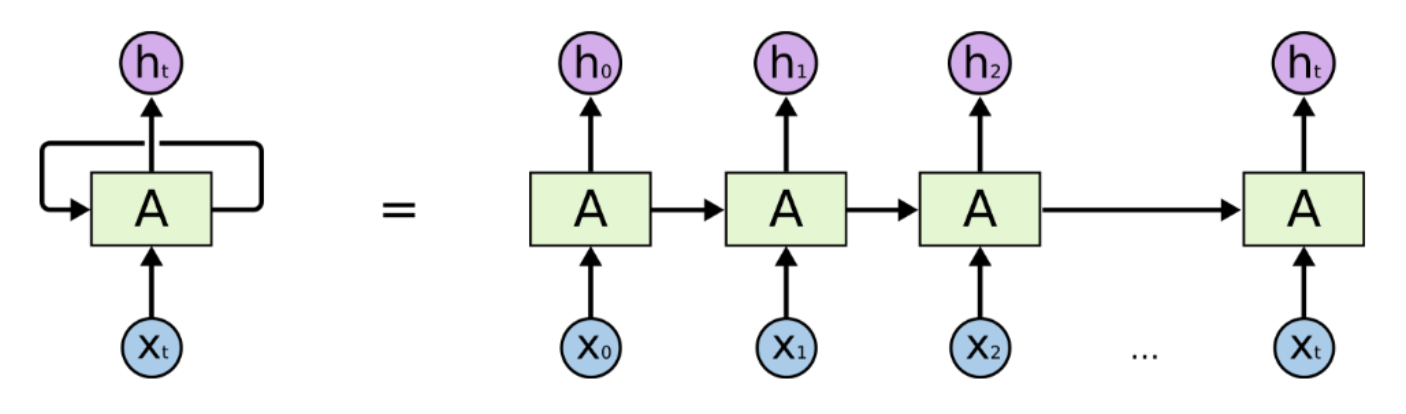
\includegraphics[width=0.7\textwidth]{figures/rnn.png}
\end{center}
\footnote{\tiny Image credit: Chris Olah~\url{https://colah.github.io/posts/2015-08-Understanding-LSTMs/}}
\end{frame}

\begin{frame}{Gradient vanishing}
\begin{itemize}
  \item<+-> Every iteration, we multiply the hidden state $h_{t-1}$ from the previous iteration with the same $W$. Recall the definition of Jacobian.
  \item<+-> If the largest singular value of $W$ is less than one then back-propagation will be attenuated.
  \item<+-> Similarly, we apply $\tanh$ activation every iteration -- further reducing gradient flow.
\end{itemize}
\begin{center}
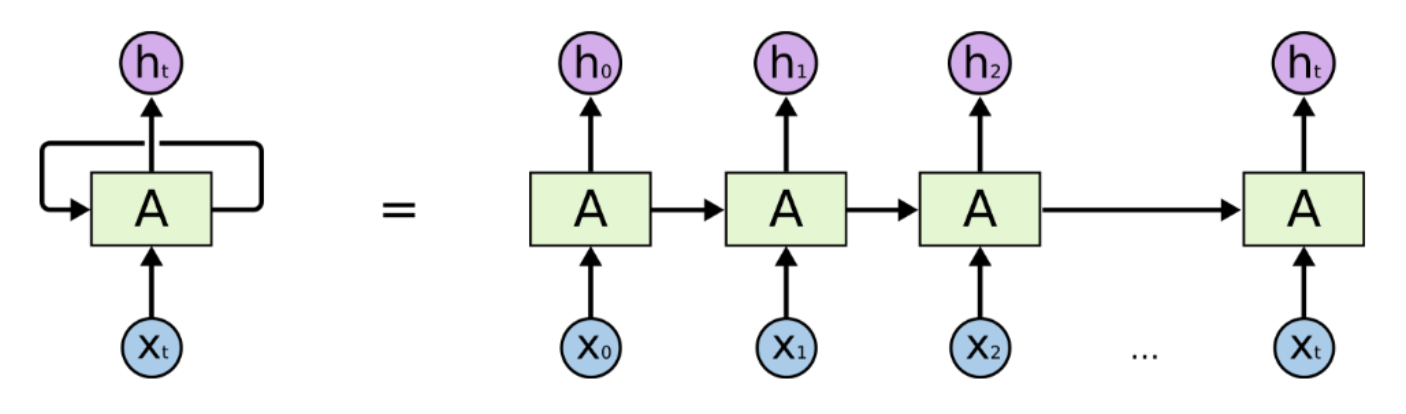
\includegraphics[width=0.7\textwidth]{figures/rnn.png}
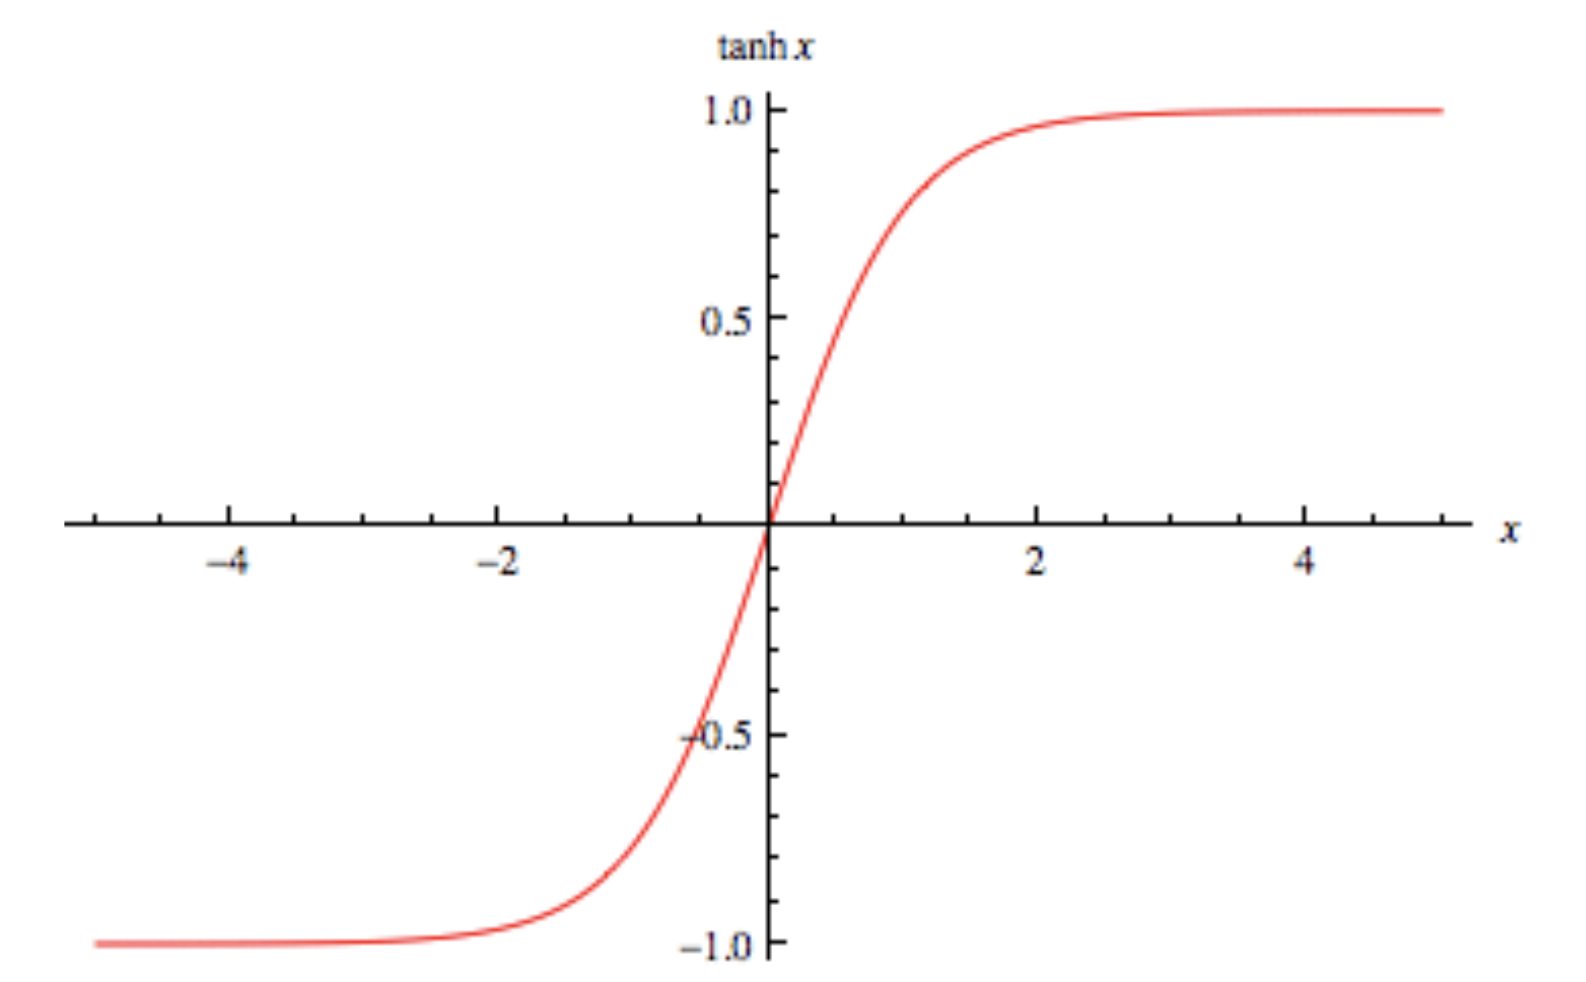
\includegraphics[width=0.25\textwidth]{figures/tanh.png}
\end{center}
\end{frame}

\begin{frame}{Gating functions in LSTM}
\begin{itemize}
    \item<+-> Long short-term memory is a network that addresses the gradient vanishing problem by introducing gating functions.
    \item<1-> Gating functions provide ``shortcuts'', like ResNet.
    \item<+-> Originally proposed by Hochreiter and Schmidhuber in 1997.
\end{itemize}
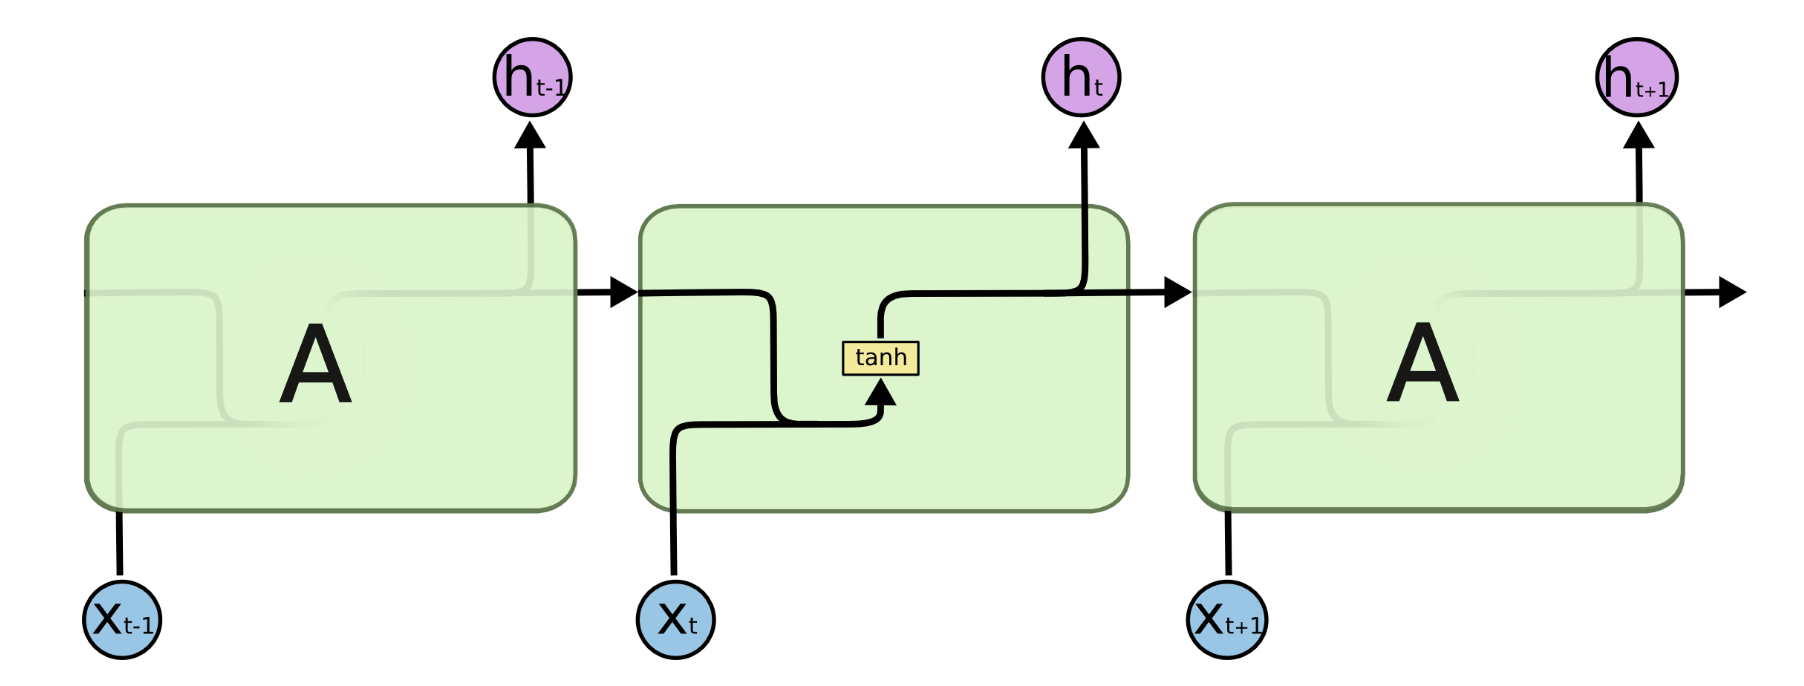
\includegraphics[width=0.49\textwidth]{figures/rnn_cell.png}
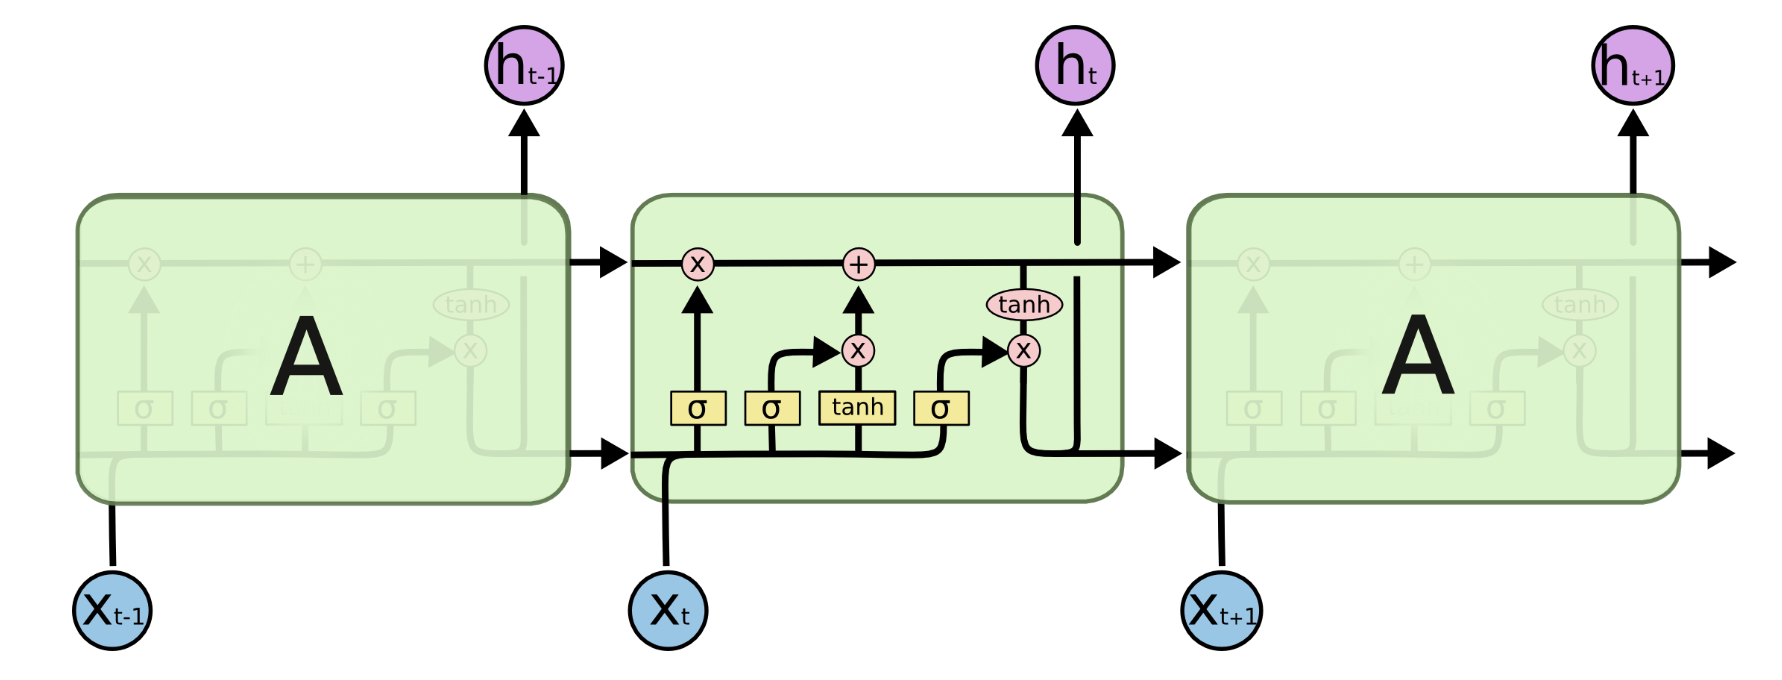
\includegraphics[width=0.49\textwidth]{figures/lstm_cell.png}
\end{frame}

\begin{frame}{Gating functions in LSTM}
\begin{columns}
\begin{column}{0.5\textwidth}
\begin{itemize}
    \item<+-> Input gate: $i_t = \sigma(W_i [h_{t-1}, x_t] + b_i)$.
    \item<1-> Forget gate: $f_t = \sigma(W_f [h_{t-1}, x_t] + b_f)$.
    \item<1-> $z_t = \tanh(w_z [h_{t-1} x_t] + b_z)$.
    \item<+-> $c_t = f_t \odot c_{t-1} + i_t \odot z_t$.
    \item<+-> Output gate: $o_t = \sigma(W_o [h_{t-1}, x_t] + b_o)$.
    \item<3-> $h_t = o_t \odot \tanh(c_t)$.
\end{itemize}
\end{column}
\begin{column}{0.5\textwidth}
\begin{center}
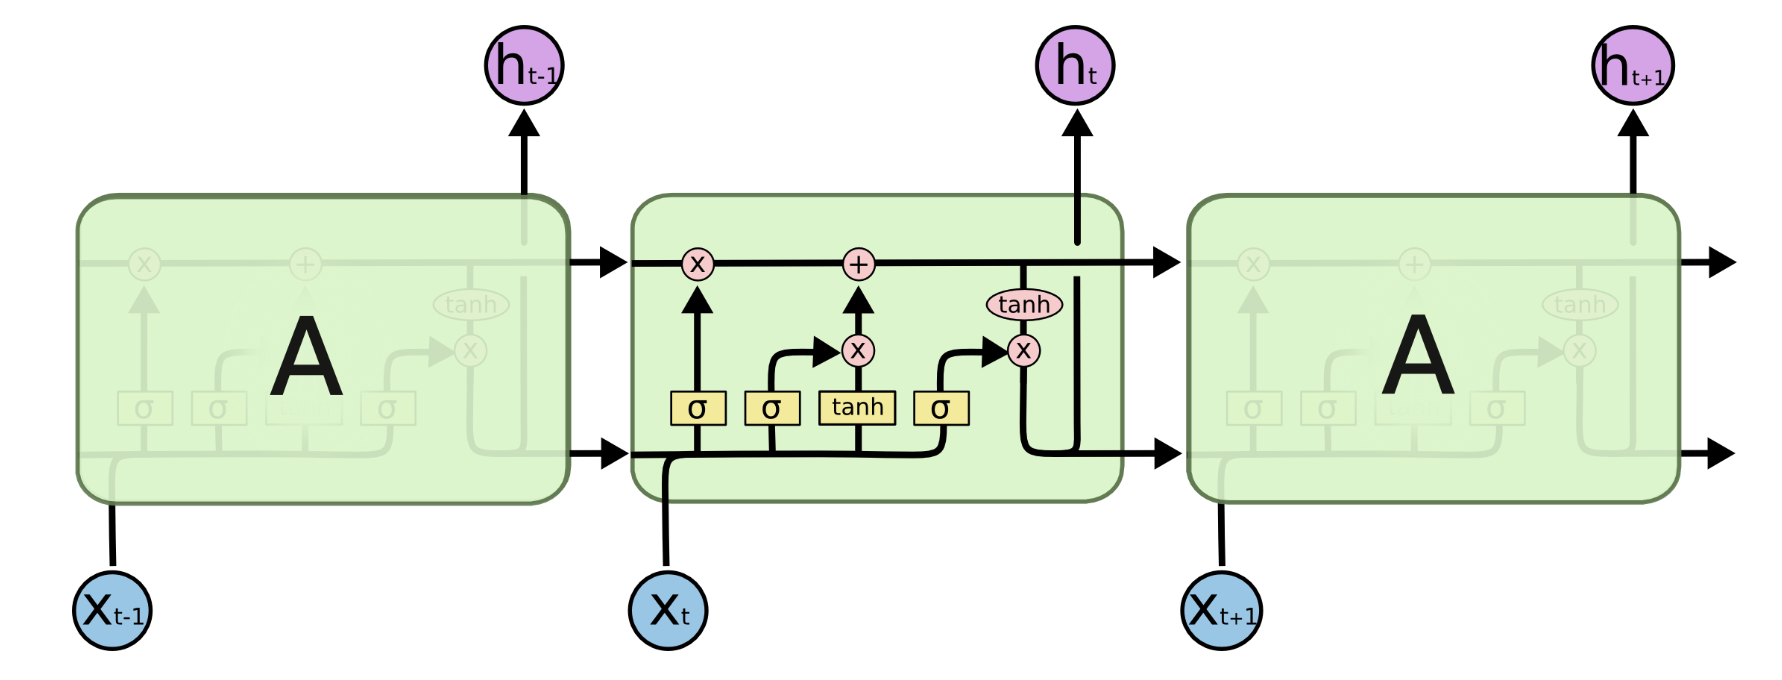
\includegraphics[width=\textwidth]{figures/lstm_cell.png}
\end{center}
\end{column}
\end{columns}
\end{frame}

\begin{frame}{Gated Recurrent Unit}
\begin{columns}
\begin{column}{0.5\textwidth}
\begin{itemize}
    \item<+-> Proposed by Chung et al. in 2015, a simplified variant compared to LSTM.
    \item<+-> Input gate $i_t = \sigma(W_i [h_{t-1}, x_t] + b_i)$.
    \item<+-> Reset gate $r_t = \sigma(W_r [h_{t-1}, x_t] + b_r)$.
    \item<+-> $\tilde{h}_t = \tanh(W_h [r_t \odot h_t, x_t] + b_h)$.
    \item<+-> $h_t = (1-i_t) \odot h_{t-1} + i_t \odot \tilde{h}_t$.
\end{itemize}
\end{column}
\begin{column}{0.5\textwidth}
\begin{center}
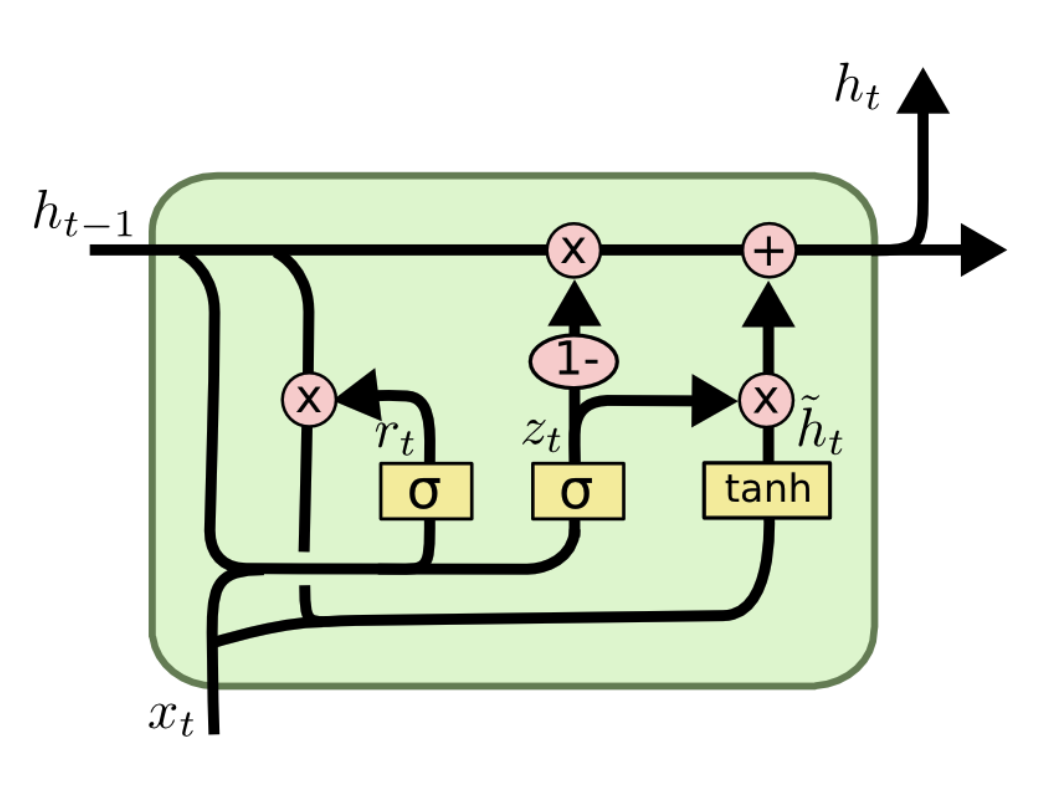
\includegraphics[width=\textwidth]{figures/gru_cell.png}
\end{center}
\end{column}
\end{columns}
\end{frame}

\begin{frame}{Attention Mechanisms}
\begin{columns}
\begin{column}{0.5\textwidth}
\begin{itemize}
    \item Earlier content will decay more.
    \item Hard to refer back to the raw content.
    \item<+-> Reverse order better than forward order [abcde -> a'b'c'd'e' vs. abcde -> e'd'c'b'a'].
    \item<+-> Attending to arbitrary sequence tokens.
    \item<+-> $s_t = f(s_{t-1}, y_{t-1}, c_t)$
    \item<+-> $c_t = \sum_\tau \alpha_{t, \tau} h_\tau$, $\alpha_{t,\tau} = \frac{\exp(a(s_{t-1},h_k))}{\sum_{k} \exp(a(s_{t-1},h_k))}$
    \item<+-> $a(s_{t-1}, h_k) = v_a^\top \tanh(W_a [s_{i-1}, h_k])$
\end{itemize}
\end{column}
\begin{column}{0.5\textwidth}
\begin{center}
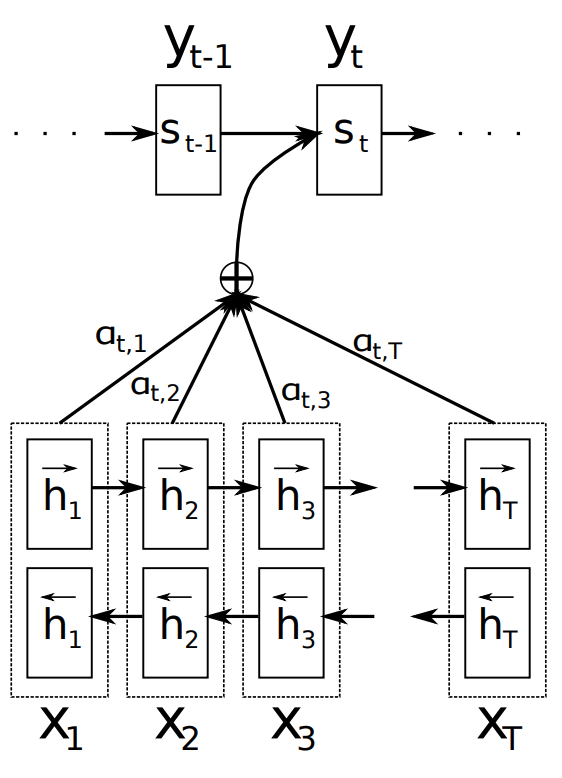
\includegraphics[width=0.6\textwidth]{figures/attention_nmt.png}\\
Bahdanau et al., 2014
\end{center}
\end{column}
\end{columns}
\end{frame}

\begin{frame}{Transformers (``Attention is All You Need'')}
\begin{itemize}
    \item<+-> The previous architecture is very complicated.
    {\small
    \begin{itemize}
    \item 1 RNN for encoding the tokens.
    \item Attention mechanisms for accessing content
    \item 1 RNN for combining attended tokens.
    \end{itemize}
    }
    \item<+-> RNNs have the ability to incorporate past information, so does attention.
    % \item Just attention is sufficient.
\end{itemize}
\begin{center}
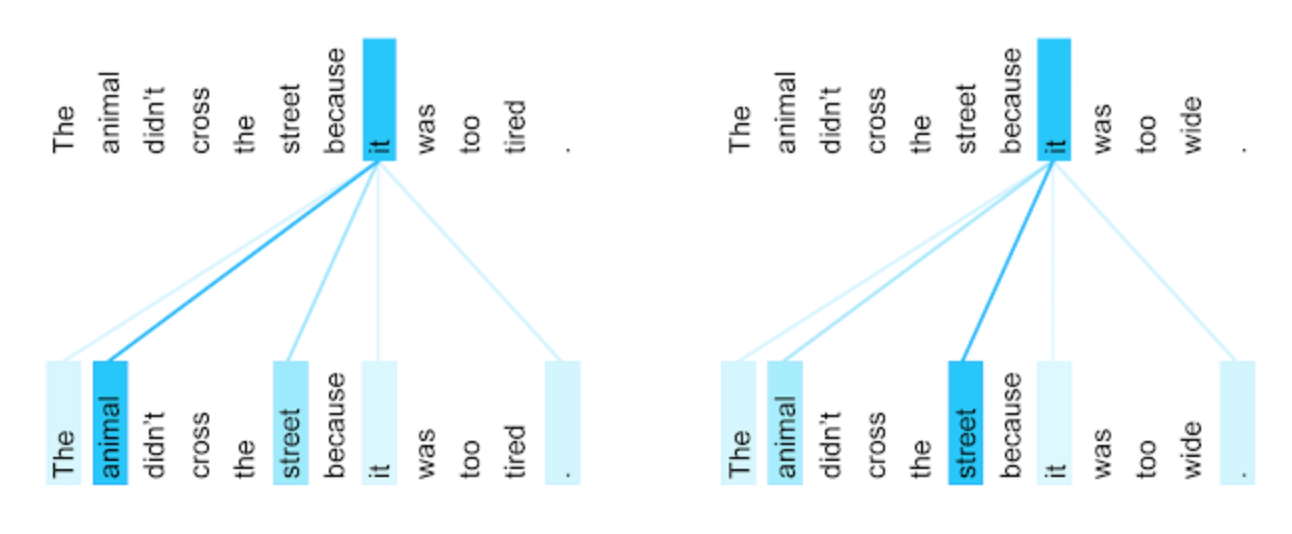
\includegraphics[width=0.4\textwidth]{figures/transformer_attention.png}\\
\footnote{\tiny Image credit: \href{https://blog.research.google/2017/08/transformer-novel-neural-network.html}{Google Research Blog}}
\end{center}
\end{frame}

\begin{frame}{Positional encoding}
\begin{itemize}
  \item Attention operation is permuation equivariant.
  \pause
  % \item We need to encode the sequence order information in the inputs.
  \item Solution: Encode the position of each token.
  \pause
  \item $PE(pos, 2i) = \sin(p/k^{2i/d}), PE(pos, 2i+1) = \cos(p/k^{2i/d})$.
\end{itemize}
\begin{center}
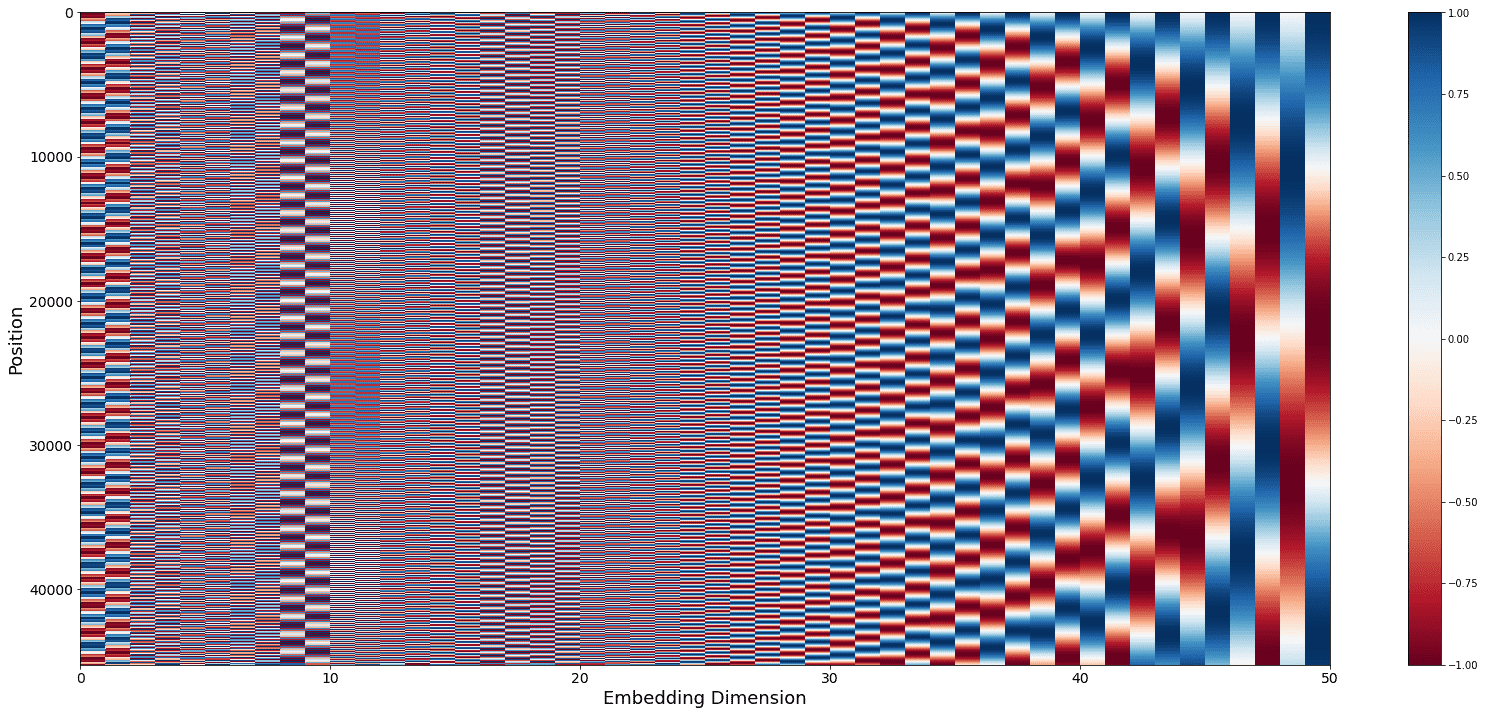
\includegraphics[width=0.6\textwidth]{figures/position_encoding.png}
\end{center}
\end{frame}

\begin{frame}{Multi-headed attention}
\begin{columns}
\begin{column}{0.5\textwidth}
\begin{itemize}
    \item<+-> Map tokens into query, key, and value.
    \item<+-> $Attention(Q,K,V)=\softmax(\frac{Q K^\top}{\sqrt{d_k}})V$.
    \item<+-> $H_i = Attention(Q W_i^Q, K W_i^K, V W_i^V)$.
    \item<+-> $MultiHead(Q, K, V) = [H_1, ..., H_n] W^O$
    % \item<+-> The vanilla form of attention in Bahdanau et al. only considers a single set of softmax values.
    \item<+-> More advantageous to have multiple set of attentions for each token, so it can more efficiently incorporate information from multiple sources.
\end{itemize}
\end{column}
\begin{column}{0.5\textwidth}
\begin{center}
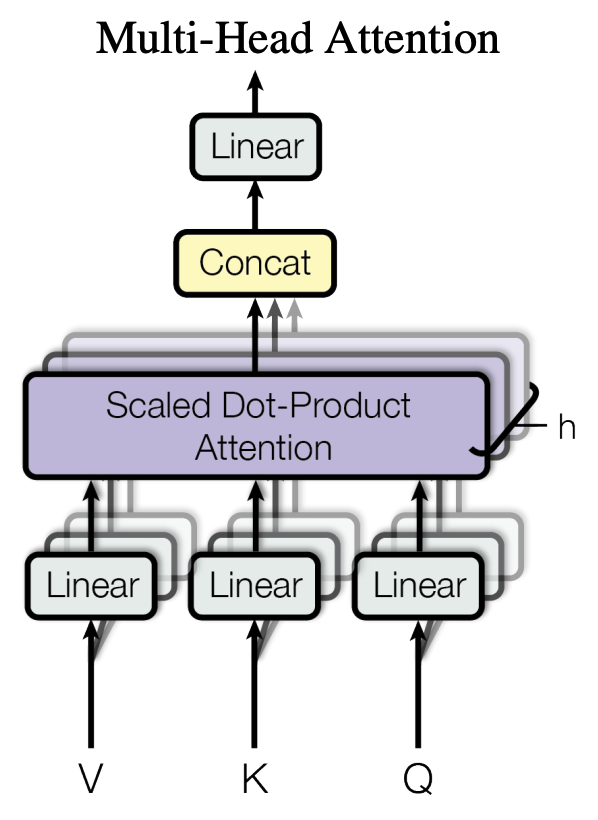
\includegraphics[width=0.5\textwidth]{figures/multi_headed_attention.png}
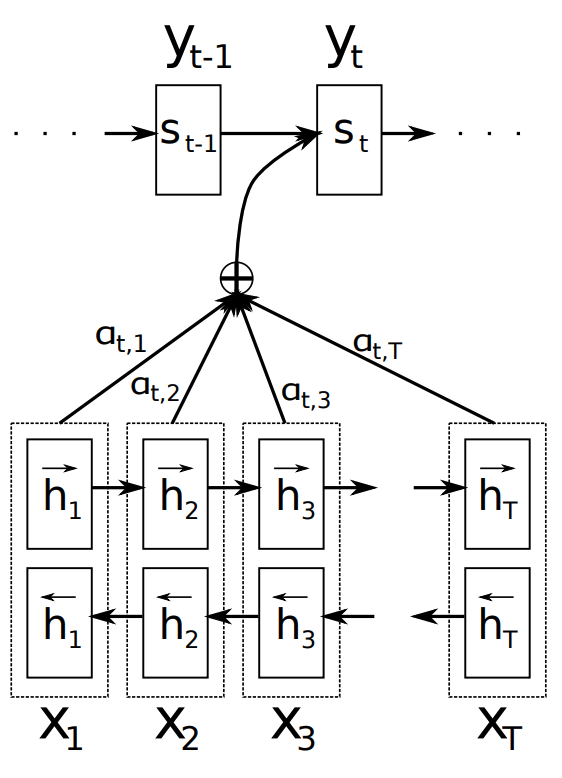
\includegraphics[width=0.45\textwidth]{figures/attention_nmt.png}
\end{center}
\end{column}
\end{columns}
\end{frame}

% \begin{frame}{Machine Translation}
% \begin{itemize}
%   \item Achieved superior performance on machine translation.
%   \item Animation \href{https://3.bp.blogspot.com/-aZ3zvPiCoXM/WaiKQO7KRnI/AAAAAAAAB_8/7a1CYjp40nUg4lKpW7covGZJQAySxlg8QCLcBGAs/s1600/transform20fps.gif}{link}
% \end{itemize}
% \begin{center}
% 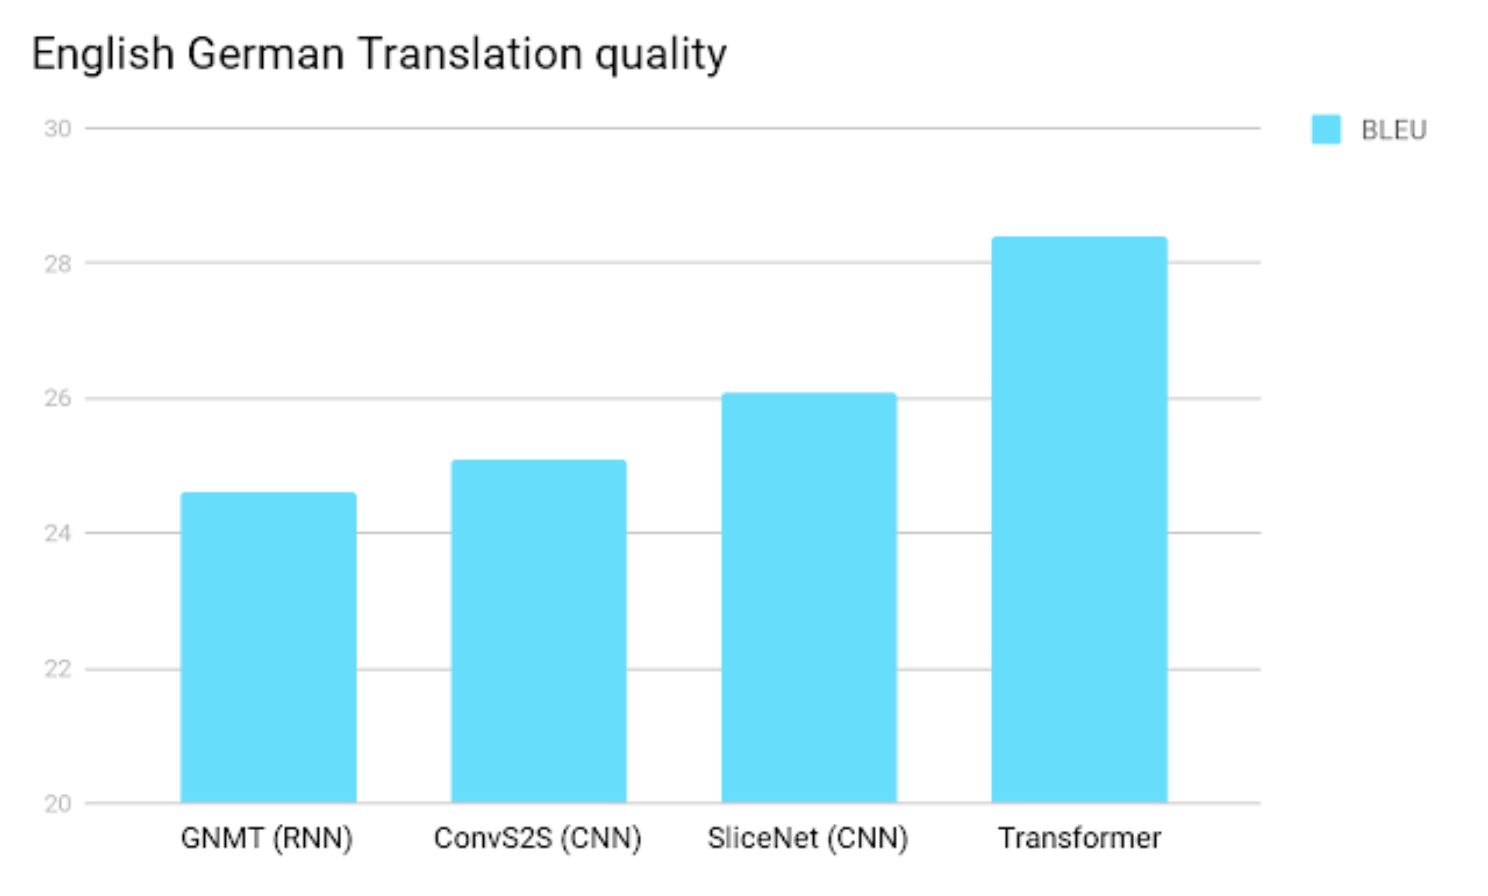
\includegraphics[height=4cm]{figures/en_de.png}
% \quad
% \includegraphics[height=4cm]{figures/en_fr.png}
% \end{center}
% \end{frame}

% \begin{frame}{Autoregressive modeling}
% \begin{itemize}
%     \item<+-> Recall the chain rule on joint distribution:
%     \[
%     p(x_{1:t}) = p(x_1, \dots, x_t) = p(x_1) p(x_2 | x_1) \dots p(x_t | x_{t-1}) = p(x_1) \prod_i p(x_i|x_{1:i-1}).
%     \]
%     \item<+-> In Naive Bayes, we treat each variable as independent, but this cannot perform sequence generation.
%     \item<+-> How do we model a conditional distribution $p(x_i|x_{1:i-1})$ using an RNN or a Transformer?
%     \item<+-> RNN is naturally autoregressive: $h_t$ contains all information up to time t.
%     \item<+-> For Transformers, $h_t$ contains information about the future.
% \end{itemize}
% \end{frame}

% \begin{frame}{Causal Attention}
%   \begin{itemize}
%     \item For Transformers, we need to ``mask'' the attention so that each token can only attend to tokens prior to itself.
%     \item This is called ``causal attention''.
%   \end{itemize}
%   \begin{center}
%   \includegraphics[width=0.7\textwidth]{figures/attention_graph.png}
%   \end{center}
%     \footnote{\tiny Image credit: \href{https://www.wolfram.com/language/12/neural-network-framework/use-transformer-neural-nets.html}{Wolfram.com}}
% \end{frame}

% \begin{frame}{Large Language Models}
% \begin{itemize}
%   \item Most LLMs today are large-scale decoder-only autoregressive (causal) Transformers (>1B parameters).
% \end{itemize}
% \begin{center}
% \includegraphics[width=0.7\textwidth]{figures/llm.png}
% \footnote{\tiny Image credit: \href{https://medium.com/@thedatabeast/top-free-courses-on-large-language-models-abf2722d15c5}{Medium.com}}
% \end{center}
% \end{frame}

\begin{frame}{Interim Summary}
\begin{itemize}
  % \item A chunk of deep learning literature in the past 10 years focuses on better optimization, reduce overfitting, and architecture motifs.
  \item<+-> Optimization: Learning rate, initialization, activation functions, normalization, shortcut skip connection, attention, etc.
  \item<+-> Overfitting: Dropout, Data augmentation, etc.
  \item<+-> Architecture Motifs: MLP, CNN, RNN, Transformers, etc.
  \item<+-> Why deep learning works? Data, optimization, compute.
  \item<+-> Still many open questions: Interpretability, fairness, uncertainty, data efficiency, energy efficiency, theory, etc.
\end{itemize}
\end{frame}

\section{Interpretability in Deep Neural Networks}

\begin{frame}{ML Interpretability}
\begin{itemize}
  \item<+-> Linear regression: Weights represent feature selection strength.
  \item<+-> SVMs: Dual weights represent sample selection.
  \item<+-> Bayesian methods: Model the generative process as a probabilistic model, fully transparent.
  \item<+-> Decision trees: If-else decision making process.
  \item<+-> Neural networks: ?
\end{itemize}
\end{frame}

\begin{frame}{Feature Visualization}
\begin{itemize}
  \item Recall: we can understand what first-layer features are doing by visualizing the weight matrices.
  \begin{center}
    \begin{columns}
      \begin{column}{0.35 \textwidth}
        \begin{center}
          Fully connected
          \includegraphics[width=0.6 \textwidth]{figures/mnist_filters.png}
        \end{center}
      \end{column}
      \begin{column}{0.35 \textwidth}
        \begin{center}
          Convolutional
          \includegraphics[width=0.55 \textwidth]{figures/zeiler_filters.pdf}
        \end{center}
        \begin{flushright}
  \tiny{Zeiler and Fergus, Visualizing and understanding convolutional networks, ECCV 2014.}
        \end{flushright}
      \end{column}
    \end{columns}
  \end{center}
\item The better the input matches these weights, the more the feature activates.
\item Higher-level weight matrices are hard to interpret.
\begin{itemize}
  \item Obvious generalization: visualize higher-level features by seeing what inputs activate them.
\end{itemize}
\end{itemize}
\end{frame}

\begin{frame}{Feature Visualization}
\begin{itemize}
\item One way to formalize: pick the images in the training set which activate a unit most strongly.
\item Here's the visualization for layer 1:
  \begin{center}
    \includegraphics[width=0.3 \textwidth]{figures/layer1.png}
  \end{center}
\end{itemize}
\begin{flushright}
  \tiny{Zeiler and Fergus, Visualizing and understanding convolutional networks, ECCV 2014.}
\end{flushright}
\end{frame}

\begin{frame}{Feature Visualization}
\begin{itemize}
\item Layer 3:
  \begin{center}
    \includegraphics[width=0.4 \textwidth]{figures/layer3.png}
  \end{center}
\end{itemize}
\begin{flushright}
  \tiny{Zeiler and Fergus, Visualizing and understanding convolutional networks, ECCV 2014.}
\end{flushright}
\end{frame}

\begin{frame}{Feature Visualization}
\begin{itemize}
\item Layer 4:
  \begin{center}
    \includegraphics[width=0.3 \textwidth]{figures/layer4.png}
  \end{center}
\end{itemize}
\begin{flushright}
  \tiny{Zeiler and Fergus, Visualizing and understanding convolutional networks, ECCV 2014.}
\end{flushright}
\end{frame}

\begin{frame}{Feature Visualization}
\begin{itemize}
\item Layer 5:
  \begin{center}
    \includegraphics[width=0.55 \textwidth]{figures/layer5.png}
  \end{center}
\end{itemize}
\begin{flushright}
  \tiny{Zeiler and Fergus, Visualizing and understanding convolutional networks, ECCV 2014.}
\end{flushright}
\end{frame}

\begin{frame}{Feature Visualization}
\begin{itemize}
  \item<+-> Higher layers seem to pick up more abstract, high-level information.
  \item<+-> Problems?
    \begin{itemize}
    \item<+->  Can't tell what the unit is actually responding to in the image.
    \item<+->  We may read too much into the results, e.g.~a unit may detect red, and the images that maximize its activation will all be stop signs.
    \end{itemize}
  \item<+-> Can use input gradients to diagnose what the unit is responding to.
\end{itemize}
\end{frame}

\begin{frame}{Feature Visualization}
\begin{itemize}
\item Input gradients can be hard to interpret.
\item Take a good object recognition conv net (Alex Net) and compute the gradient of $\log p(y= \textrm{``cat''} | \mathbf{x})$:
  \begin{center}
    \begin{columns}
      \begin{column}{0.35 \textwidth}
        \begin{center}
          Original image
          \includegraphics[width=0.8 \textwidth]{figures/cat.pdf}
        \end{center}
      \end{column}
      \begin{column}{0.35 \textwidth}
        \begin{center}
          Gradient for ``cat''
          \includegraphics[width=0.7 \textwidth]{figures/cat_gradient.pdf}
        \end{center}
      \end{column}
    \end{columns}
  \end{center}
\end{itemize}
\end{frame}

\begin{frame}{Feature Visualization}
  \begin{itemize}
  \item \alert{Guided backprop} is a total hack to prevent this cancellation.
  \item Do the backward pass as normal, but apply the ReLU nonlinearity to all the activation error signals.
    \[ y = \textrm{ReLU}(z) \qquad \bar{z} = \begin{cases} \bar{y} & \text{if $z > 0$ {\color{red} and $\bar{y} > 0$}} \\ 0 & \text{otherwise} \end{cases} \]
  \item We want to visualize what excites given unit, not what suppresses it.
    \begin{center}
      \includegraphics[width=0.45 \textwidth]{figures/guided_backprop_results.pdf}
    \end{center}
  \end{itemize}
\end{frame}

\begin{frame}{Guided Backprop}
\begin{center}
  \includegraphics[width=0.7 \textwidth]{figures/guided_backprop_results2.pdf}
\end{center}
\begin{flushright}
{\tiny Springerberg et al., Striving for simplicity: The all convolutional net, ICLR workshop 2015.}
\end{flushright}

% \notenew{
% \begin{itemize}
%   \item We start from here.
%   \item Visualize one neuron in the input image.
%   \item Draw one neuron in the middle.
% \end{itemize}
% }
\end{frame}


\begin{frame}{Class activation map (CAM)}

\begin{itemize}
\item Classification networks typically use global avg pooling before the final layer.

\item This pooling layer can already contain semantic information.

\item We can visualize a heat map 
\end{itemize}

\begin{center}
\includegraphics[height=0.3\textheight]{figures/cam.png}
\includegraphics[height=0.3\textheight]{figures/cam2.png}
\end{center}

\begin{flushright}
{\tiny Zhou et al. Learning deep features for discriminative localization. CVPR 2016.}
\end{flushright}

% \notenew{
%   \begin{itemize}
%     \item Another way is to think about the output classes.
%     \item Imagine you have a classifier.
%     \item What would be the region of the input that is responsible 
%     \item Utilize the average pooling layer.
%     \item Take the dot product between the activation at each location and the class vector
%   \end{itemize}
% }
\end{frame}

\begin{frame}{GradCAM}

\begin{center}
% \vspace{-0.2in}
\includegraphics[width=0.9\textwidth]{figures/gradcam.png}
\end{center}

\begin{flushright}
{\tiny Selvaraju et al. Grad-CAM: Visual explanations from deep networks via gradient-based localization. ICCV 2017.}
\end{flushright}

% \notenew{
%   \begin{itemize}
%     \item Potentially a way to combine guided backprop and CAM.
%     \item In the example, GBP is still plotting the dog, even though we are visualizing the cat neuron.
%     \item We can suppress it by overlapping it with CAM.
%   \end{itemize}
% }
\end{frame}

\begin{frame}{GradCAM}
\begin{center}
\includegraphics[width=0.8\textwidth,trim={0 0 16cm 0},clip]{figures/gradcam2.png}
\end{center}
\begin{flushright}
{\tiny Selvaraju et al. Grad-CAM: Visual explanations from deep networks via gradient-based localization. ICCV 2017.}
\end{flushright}
\end{frame}

\begin{frame}{DeepDream\footnote{\tiny \href{https://blog.research.google/2015/07/deepdream-code-example-for-visualizing.html?m=1}{Google Research Blog}}}
\begin{itemize}
\item Start with an image, and run a conv net on it.
\item Change the image such that units which were already highly activated get activated even more strongly.
``Rich get richer.''
\end{itemize}
\begin{center}
  \hspace{-1em}\includegraphics[width=0.9\textwidth]{figures/deepdream1.pdf}
\end{center}

% \notenew{
% \begin{itemize}
%   \item What if we try to maximize all neuron in one layer at once?
% \end{itemize}
% }
\end{frame}

\begin{frame}{DeepDream}
\begin{center}
  \hspace{-1em}\includegraphics[width=0.9\textwidth]{figures/deepdream2.pdf}
\end{center}
\end{frame}

\begin{frame}{DeepDream}
\begin{center}
  \hspace{-1em}\includegraphics[width=0.7\textwidth]{figures/deepdream3.pdf}
\end{center}
\end{frame}

\begin{frame}{Gradient Ascent on Images}
\begin{itemize}
\item Doing gradient ascent on an image to maximize the activation of a given neuron.
  \begin{center}
    \hspace{-3em}\includegraphics[width=\textwidth]{figures/distill_gd.png}
  \end{center}
\end{itemize}
\begin{flushright}
  \begin{tiny}
    \vspace{-1em}
    \url{https://distill.pub/2017/feature-visualization/}
  \end{tiny}
\end{flushright}

% \notenew{
%   \begin{itemize}
%     \item Guided backpropagation = 1 step
%     \item What if we run multiple steps of gradients?
%   \end{itemize}
% }
\end{frame}

\begin{frame}{Gradient Ascent on Images}
\begin{center}
  \hspace{-1em}\includegraphics[width=\textwidth]{figures/distill_why_optimize.png}
\end{center}
\begin{flushright}
  \begin{tiny}
    \vspace{-1em}
    \url{https://distill.pub/2017/feature-visualization/}
  \end{tiny}
\end{flushright}

% \notenew{
%   \begin{itemize}
%     \item For the same layer, we can run it on different units, and get different results.
%     \item Above: dataset examples that maximizes neuron activation
%     \item Below: optimized images that maximizes neuron activation
%   \end{itemize}
% }
\end{frame}

\begin{frame}{Gradient Ascent on Images}
\begin{itemize}
  \item Higher layers in the network often learn higher-level, more interpretable representations
    \begin{center}
      \includegraphics[width=0.85 \linewidth]{figures/olah.png}
    \end{center}
    \begin{flushright}
      \begin{tiny}
        \vspace{-1em}
        \url{https://distill.pub/2017/feature-visualization/}
      \end{tiny}
    \end{flushright}
\end{itemize}
\end{frame}

\begin{frame}{Gradient Ascent on Images}
\begin{itemize}
  \item Higher layers in the network often learn higher-level, more interpretable representations
    \begin{center}
      \includegraphics[width=0.6 \linewidth]{figures/olah2.png}
    \end{center}
    \begin{flushright}
      \begin{tiny}
        \vspace{-1em}
        \url{https://distill.pub/2017/feature-visualization/}
      \end{tiny}
    \end{flushright}
\end{itemize}
\end{frame}


\begin{frame}{Artistic style transfer}
\begin{itemize}
\item Activations store content information
\item Activation correlation stores style/texture information: $G^{l}_{ij} = \sum_k F^{l}_{ik} F^{l}_{jk}$
\end{itemize}
\begin{center}
\includegraphics[width=0.45\textwidth]{figures/style_transfer.png}
\end{center}
\begin{flushright}
{\tiny Gatys et al., Image style transfer using convolutional neural networks, CVPR 2016.}
\end{flushright}

% \notenew{
%   \begin{itemize}
%     \item Backprop into the inputs can generate a lot of interesting patterns.
%     \item This could include low level image patterns.
%     \item What about change the style of an image?
%   \end{itemize}
% }
\end{frame}

\begin{frame}{Artistic style transfer}
\begin{itemize}
  \item Optimizing both content \& style from random noise
\end{itemize}
\begin{center}
\includegraphics[width=0.65\textwidth]{figures/style_transfer2.png}
\end{center}
\begin{flushright}
{\tiny Gatys et al., Image style transfer using convolutional neural networks, CVPR 2016.}
\end{flushright}
\end{frame}

\begin{frame}{Artistic style transfer}
\begin{center}
\includegraphics[width=0.55\textwidth,trim={0 7cm 0 0},clip]{figures/style_transfer3.png}
\end{center}
\begin{flushright}
{\tiny Gatys et al., Image style transfer using convolutional neural networks, CVPR 2016.}
\end{flushright}
\end{frame}

\begin{frame}{Adversarial Examples}
\begin{itemize}
\item One of the most surprising findings about neural nets has been the existence of \alert{adversarial inputs}, i.e.~inputs optimized to fool an algorithm.
\end{itemize}
\begin{center}
    \includegraphics[width=0.75 \linewidth]{figures/fgsm.png}
  \end{center}
\begin{flushright}
  \tiny{Goodfellow et al., Explaining and harnessing adversarial examples, ICLR 2015.}
\end{flushright}
% \notenew{
%     Given an image for one category (e.g.~``cat''), compute the image gradient to maximize the network's output unit for a different category (e.g.~``dog'')
%     \begin{itemize}
%       \item Perturb the image very slightly in this direction
%       \item Works slightly better if you take the sign of the entries in the gradient; this is called the \high{fast gradient sign method}.
%     \end{itemize}
% }
\end{frame}

\begin{frame}{Adversarial Examples}
\begin{itemize}
\item The following adversarial examples are misclassified as ostriches. ( $10 \times$ perturbation visualized in middle.)
  \begin{center}
    \includegraphics[width=0.85 \linewidth]{figures/adversarial_examples.png}
  \end{center}
\end{itemize}
\begin{flushright}
  \tiny{Szegedy et al., Intriguing properties of neural networks, ICLR 2014.}
\end{flushright}
\end{frame}

\begin{frame}{Adversarial Examples}
\begin{itemize}
\item You can print out an adversarial image and take a picture of it, and it still works!
  \begin{center}
    \includegraphics[width=0.9 \linewidth]{figures/printed_adversarial.png}
  \end{center}
  \begin{flushright}
    \tiny{Kurakin et al., Adversarial examples in the physical world, ICLR workshop 2017.}
  \end{flushright}
\end{itemize}
\end{frame}

\begin{frame}{Adversarial Examples}
\begin{itemize}
\item An adversarial example in the physical world (network thinks it's a gun, from a variety of viewing angles!)
  \begin{center}
    \includegraphics[width=0.7\textwidth]{figures/adversarial_physical.png}
  \end{center}
\end{itemize}
\begin{flushright}
  \tiny{Athalye et al., Synthesizing robust adversarial examples, ICML 2018.}
\end{flushright}
% \notenew{
%   \begin{itemize}
%   \item Optimize different view angles in 3D simulation, randomizing a lot of transformations.
%   \end{itemize}
% }
\end{frame}

\begin{frame}{Adversarial Examples}
\begin{itemize}
\item An adversarial mesh object that can hide cars from LiDAR detector
  \begin{center}
    \includegraphics[width=0.6\textwidth]{figures/adv_mesh.png}
  \end{center}
\end{itemize}
\begin{flushright}
  \tiny{Tu et al., Physically realizable adversarial examples for LiDAR object detection, CVPR 2020.}
\end{flushright}
% \notenew{
%   \begin{itemize}
%     \item People often use self-driving car as an example to emphasize the importance.
%     \item In this example, this is a 3D vision task, but the intuition is similar.
%     \item Tries to fool an object detector with a strange looking shape.
%   \end{itemize}
% }
\end{frame}

% \begin{frame}{Large Language Model Safety}
% \begin{itemize}
%   \item The vulnerability of deep networks also extend to LLMs.
%   \item People have recently come up with 
% \end{itemize}
% \end{frame}

\begin{frame}{Adversarial Defense}
\begin{itemize}
  \item<+-> How to defend from adversarial perturbation is still an active research area.
  \item<+-> Blackbox vs. whitebox attacks.
  \item<+-> One common approach is to train with millions of adversarial examples.
  \item<3-> Needs to train much longer, and also suffers a drop in accuracy.
  \item<+-> Data augmentation and label smoothing also help.
\end{itemize}
% \notenew{
%   More to be covered in security \& privacy of deep learning.
% }
\end{frame}

\begin{frame}{Summary}
\begin{itemize}
  \item<+-> Interpretability - ways to open up the black box of neural networks
  \item<+-> Knowing what each neuron does is like studying a ``brain'' with perfect observation and measurement.
  \item<+-> Still very open research area.
  \item<+-> Adversarial examples are safety vulnerabilities of deep neural networks.
  \item<+-> Need more data and innovations in more robust learning objectives.
\end{itemize}
\end{frame}
\end{document}
